\documentclass{report}
\usepackage{pdfpages}
\usepackage{graphicx} 
\usepackage{dirtytalk}
\usepackage{lmodern}
\usepackage{booktabs}
\usepackage{listings}
\usepackage{float}
\usepackage{siunitx}
\usepackage{amsmath}
\usepackage{rotating}
\usepackage{pdflscape}
\usepackage{arydshln}
\usepackage[hidelinks]{hyperref}
\usepackage[ngerman]{babel}
\usepackage[a4paper, total={6in, 8in}]{geometry}
\usepackage{caption}

\newcommand{\source}[1]{\caption*{\textit{Quelle: {#1}}} }

\begin{document}

\includepdf[pages=-]{./PDFs/Deckblatt-P2}
\begin{titlepage}
    \begin{center}
        \vspace*{1cm}
            
        \Huge
        \textbf{Auswertung und Protokoll}
            
        \vspace{0.5cm}
        \LARGE
        Zum Versuch APW
        
        \vspace{1.8cm}

        \textbf{Jonas Müther \& Alejandro Schultheiss}
        \vfill
            
        P2 Praktikum\\
       
            
        \vspace{0.8cm}
  

        \vspace{1.8cm}
        \Large
        LMU München \\
        Physik B.Sc.\\
        Deutschland\\
        2026
            
    \end{center}
\end{titlepage}
\tableofcontents

\newpage
\chapter{Vorbereitung}

\section{Versuchsvorbereitung und Grundlagen des Versuchs}
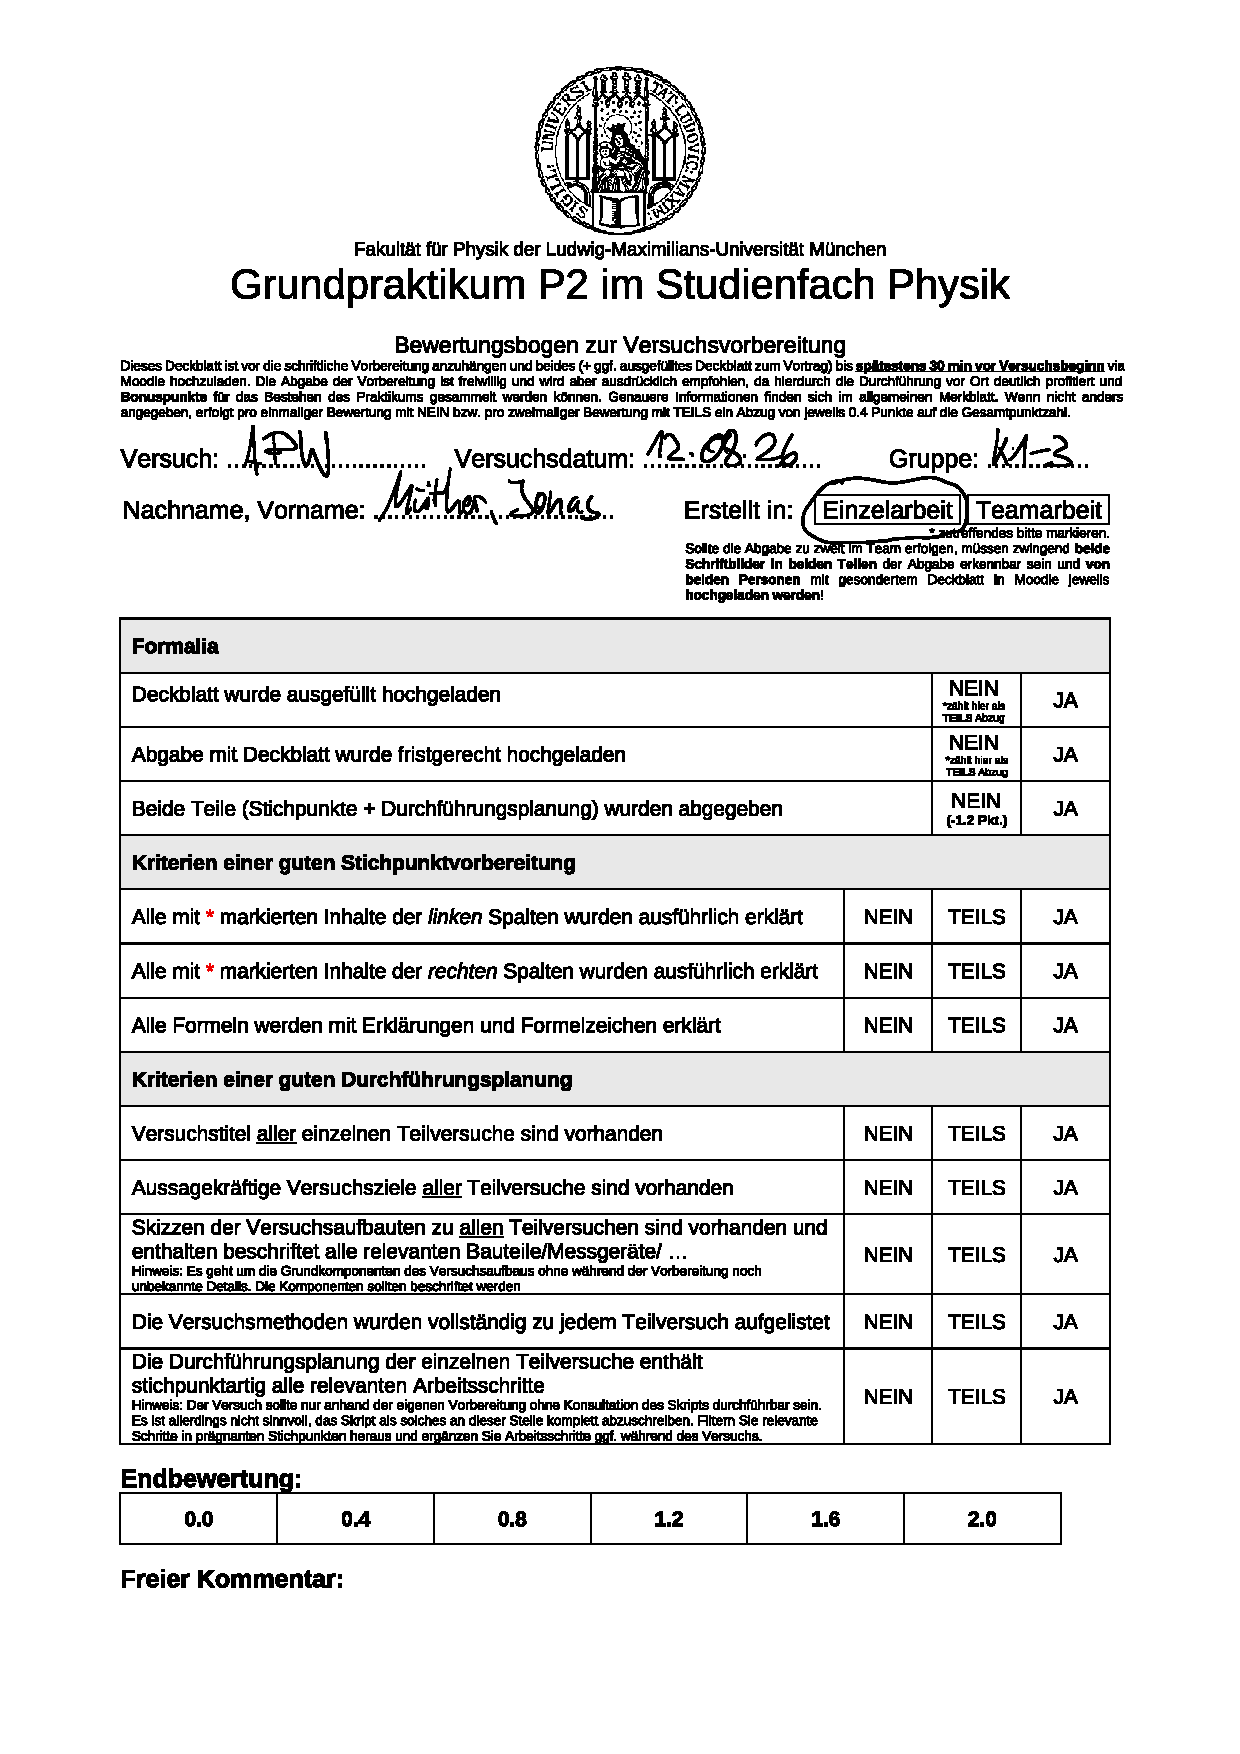
\includepdf[pages=-]{./PDFs/VorbereitungAPW.pdf}

\section{Versuchsprotokoll}
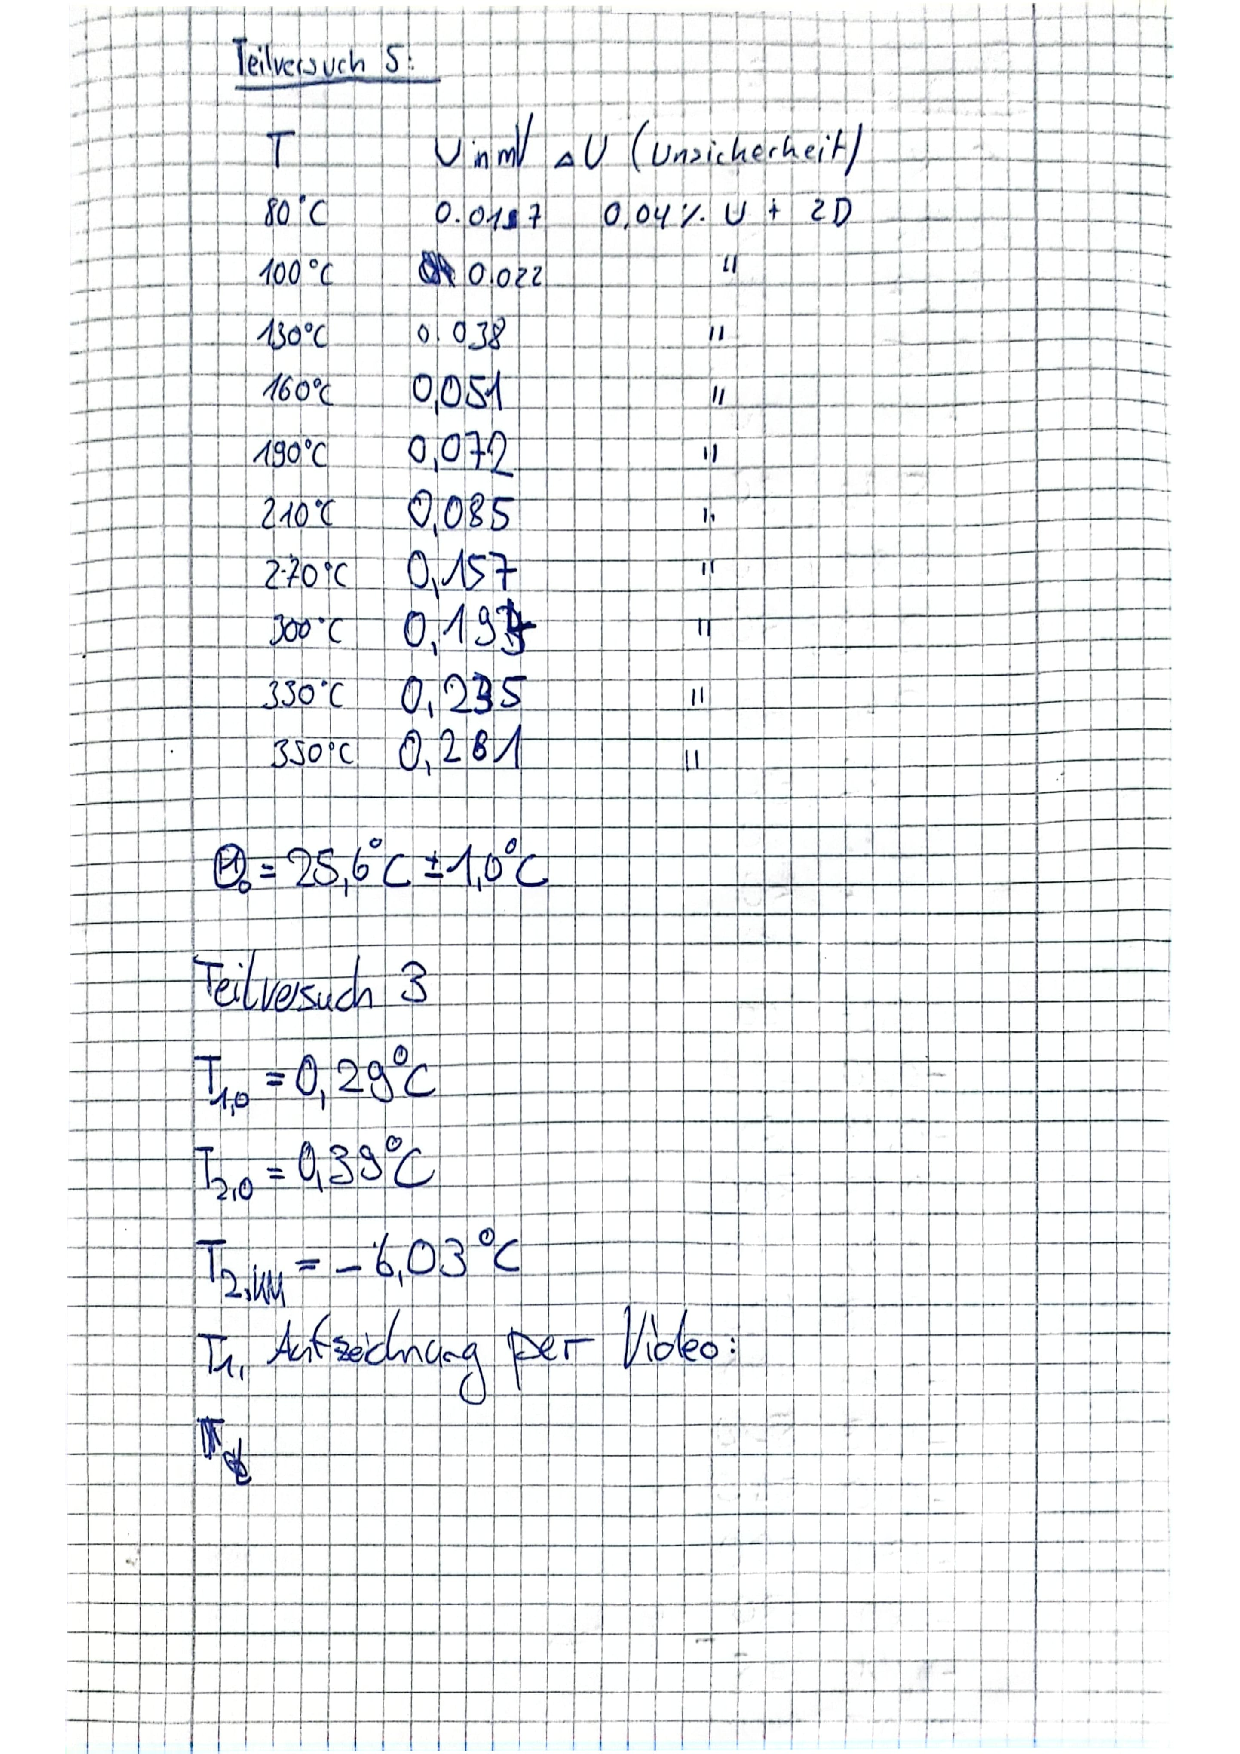
\includepdf[pages=-]{./PDFs/APWProtokoll.pdf}

\newpage
\chapter{Auswertung}
\section{Teilversuch I:}
\subsubsection{Messwerte}
\noindent
Für die Wägungen wurde eine Unsicherheit von
\[
\Delta m = \pm 0{,}04\,\mathrm{g}
\]
\noindent
angegeben. Die Unsicherheit der Temperaturmessung wird gemäß Vorgabe
vernachlässigt.
\noindent
Für die spezifische Wärmekapazität von Wasser und den Wasserwert des
Kalorimeters werden die in der Versuchsanleitung angegebenen Werte
\[
c_\mathrm{w} = 4{,}18\,\frac{\mathrm{J}}{\mathrm{g\,K}},
\qquad
m_\mathrm{w}^{*} = 80\,\mathrm{g}
\]
verwendet.
\noindent
Für die Temperatur der Probekörper unmittelbar vor dem Einsetzen in das
Kalorimeter wird nominell
\[
\Theta_\mathrm{s} = 80^\circ\mathrm{C}
\]
\noindent
angesetzt. Dabei ist zu beachten, dass die Probekörper im Temperierbad nur
ungefähr bis zur Hälfte in das Wasser eingetaucht waren.

\paragraph{Blei}
\noindent
Die Masse des Bleikörpers beträgt
\[
m_\mathrm{Pb} = (1928{,}72 \pm 0{,}04)\,\mathrm{g}.
\]
\noindent
Die Wassermasse ergibt sich aus der Differenz
\[
m_{\mathrm{w,Pb}}
=
m_{\mathrm{Becher+Wasser}}-m_{\mathrm{Becher}}
\]
zu
\[
m_{\mathrm{w,Pb}}
=
1096{,}63\,\mathrm{g}-304{,}46\,\mathrm{g}
=
792{,}17\,\mathrm{g}.
\]
\noindent
Da die Wassermasse aus zwei unabhängigen Wägungen als Differenz bestimmt
wurde, wird für die Min-Max-Methode die Größtunsicherheit
\[
\Delta m_{\mathrm{w,Pb}}
=
0{,}04\,\mathrm{g}+0{,}04\,\mathrm{g}
=
0{,}08\,\mathrm{g}
\]
\noindent
angesetzt. Somit gilt
\[
m_{\mathrm{w,Pb}}=(792{,}17\pm0{,}08)\,\mathrm{g}.
\]
\noindent
Die aufgenommene Temperatur-Zeit-Messreihe lautet:

\begin{center}
\begin{tabular}{c|c}
$t/\mathrm{s}$ & $\Theta/^\circ\mathrm{C}$\\
\hline
-20 & 27,0\\
-15 & 27,0\\
-10 & 27,1\\
-5  & 27,0\\
0   & 27,0\\
5   & 29,0\\
10  & 30,1\\
15  & 30,0\\
30  & 30,0\\
60  & 30,0\\
90  & 29,9\\
110 & 29,9\\
150 & 30,0\\
200 & 30,0\\
300 & 29,9
\end{tabular}
\end{center}

\paragraph{Aluminium}
\noindent
Die Masse des Aluminiumkörpers beträgt
\[
m_\mathrm{Al}=(488{,}03\pm0{,}04)\,\mathrm{g}.
\]
\noindent
Für die Wassermasse erhält man
\[
m_{\mathrm{w,Al}}
=
1028{,}32\,\mathrm{g}-306{,}31\,\mathrm{g}
=
722{,}01\,\mathrm{g}.
\]
\noindent
Damit gilt entsprechend
\[
m_{\mathrm{w,Al}}=(722{,}01\pm0{,}08)\,\mathrm{g}.
\]
\noindent
Die Temperatur-Zeit-Messreihe lautet:

\begin{center}
\begin{tabular}{c|c}
$t/\mathrm{s}$ & $\Theta/^\circ\mathrm{C}$\\
\hline
-20 & 27,5\\
-15 & 27,4\\
-10 & 27,5\\
-5  & 27,5\\
0   & 27,5\\
5   & 30,1\\
10  & 31,4\\
15  & 32,6\\
30  & 32,5\\
60  & 32,5\\
90  & 32,4\\
110 & 32,4\\
150 & 32,4\\
200 & 32,3\\
300 & 32,3
\end{tabular}
\end{center}


\subsubsection{Bestimmung der Mischtemperaturen}
\begin{figure}[H]
            \centering
            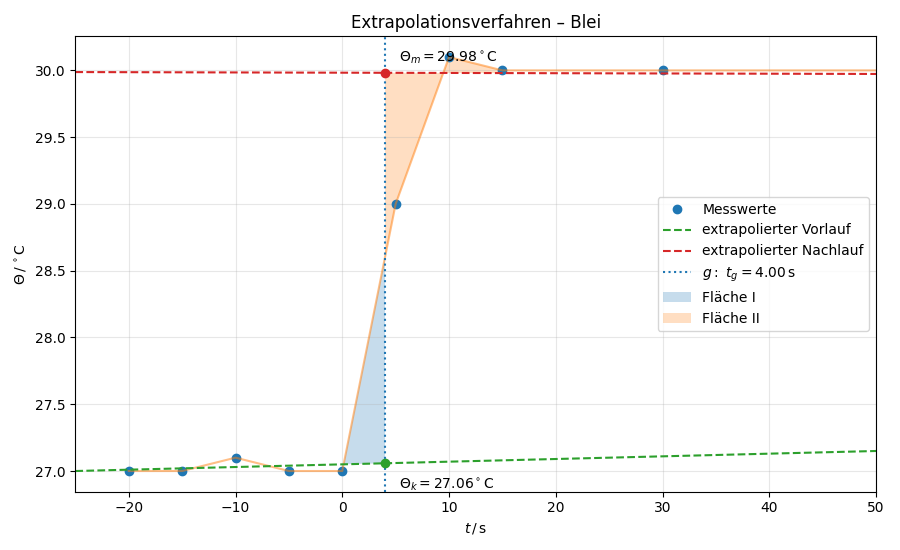
\includegraphics[width=0.8\textwidth]{./Images/Figure_3.png}
            \caption{Diagramm des Extrapolationsverfahren}
            \label{fig:StefanBoltzmann}
\end{figure}
\noindent
Da das Kalorimeter nicht ideal wärmeisoliert ist, wird die Mischtemperatur
nicht einfach mit dem höchsten gemessenen Temperaturwert gleichgesetzt.
Stattdessen werden entsprechend der Versuchsanleitung der annähernd lineare
Vorlauf und der lineare Nachlauf extrapoliert.
\noindent
Die vertikale Ausgleichsgerade wird so gewählt, dass die beiden Flächen
zwischen Messkurve und extrapolierten Geraden während des Mischvorgangs
gleich groß sind.
\noindent
Für Blei ergibt die lineare Anpassung des Vorlaufs näherungsweise
\[
\Theta_{\mathrm{V,Pb}}(t)
=
\left(
27{,}05
+
0{,}0020\,\frac{t}{\mathrm{s}}
\right)^\circ\mathrm{C},
\]
\noindent
während der Nachlauf durch
\[
\Theta_{\mathrm{N,Pb}}(t)
=
\left(
29{,}9827
-
1{,}91\cdot10^{-4}\,\frac{t}{\mathrm{s}}
\right)^\circ\mathrm{C}
\]
\noindent
beschrieben werden kann.
\noindent
Aus der Gleichflächenbedingung ergibt sich näherungsweise
\[
t_{\mathrm{g,Pb}}\approx4{,}0\,\mathrm{s}.
\]
\noindent
Die extrapolierte Anfangs- und Mischtemperatur lauten damit
\[
\boxed{\Theta_{\mathrm{k,Pb}}\approx27{,}06^\circ\mathrm{C}}
\]
und
\[
\boxed{\Theta_{\mathrm{m,Pb}}\approx29{,}98^\circ\mathrm{C}}.
\]
\noindent
Für Aluminium ergeben sich entsprechend
\[
\Theta_{\mathrm{V,Al}}(t)
=
\left(
27{,}50
+
0{,}0020\,\frac{t}{\mathrm{s}}
\right)^\circ\mathrm{C}
\]
\noindent
und
\[
\Theta_{\mathrm{N,Al}}(t)
=
\left(
32{,}508
-
8{,}04\cdot10^{-4}\,\frac{t}{\mathrm{s}}
\right)^\circ\mathrm{C}.
\]
\noindent
Die Gleichflächenbedingung liefert
\[
t_{\mathrm{g,Al}}\approx5{,}9\,\mathrm{s}.
\]
\noindent
Damit folgen
\[
\boxed{\Theta_{\mathrm{k,Al}}\approx27{,}51^\circ\mathrm{C}}
\]
und
\[
\boxed{\Theta_{\mathrm{m,Al}}\approx32{,}50^\circ\mathrm{C}}.
\]


\subsubsection{Bestimmung der spezifischen Wärmekapazitäten}
\noindent
Beim Temperaturausgleich entspricht die vom Probekörper abgegebene
Wärmemenge näherungsweise der vom Wasser und Kalorimeter aufgenommenen
Wärmemenge:
\[
Q_\mathrm{Probe}=Q_\mathrm{Kal}.
\]
\noindent
Mit
\[
Q_\mathrm{Kal}
=
c_\mathrm{w}
\left(m_\mathrm{w}+m_\mathrm{w}^{*}\right)
\left(\Theta_\mathrm{m}-\Theta_\mathrm{k}\right)
\]
\noindent
und
\[
Q_\mathrm{Probe}
=
c_\mathrm{s}m_\mathrm{s}
\left(\Theta_\mathrm{s}-\Theta_\mathrm{m}\right)
\]
\noindent
folgt
\[
c_\mathrm{s}
=
\frac{
c_\mathrm{w}
\left(m_\mathrm{w}+m_\mathrm{w}^{*}\right)
\left(\Theta_\mathrm{m}-\Theta_\mathrm{k}\right)
}{
m_\mathrm{s}
\left(\Theta_\mathrm{s}-\Theta_\mathrm{m}\right)
}.
\]


\paragraph{Blei}
\noindent
Einsetzen der gemessenen Werte mit Einheiten ergibt
\[
c_\mathrm{Pb}
=
\frac{
4{,}18\,\frac{\mathrm{J}}{\mathrm{g\,K}}
\cdot
(792{,}17\,\mathrm{g}+80\,\mathrm{g})
\cdot
(29{,}98-27{,}06)\,\mathrm{K}
}{
1928{,}72\,\mathrm{g}
\cdot
(80-29{,}98)\,\mathrm{K}
}.
\]
\noindent
Daraus folgt
\[
c_\mathrm{Pb}
=
0{,}11050\,\frac{\mathrm{J}}{\mathrm{g\,K}}.
\]


\paragraph{Aluminium}
\noindent
Analog ergibt sich
\[
c_\mathrm{Al}
=
\frac{
4{,}18\,\frac{\mathrm{J}}{\mathrm{g\,K}}
\cdot
(722{,}01\,\mathrm{g}+80\,\mathrm{g})
\cdot
(32{,}50-27{,}51)\,\mathrm{K}
}{
488{,}03\,\mathrm{g}
\cdot
(80-32{,}50)\,\mathrm{K}
}.
\]
\noindent
Damit folgt
\[
c_\mathrm{Al}
=
0{,}72187\,\frac{\mathrm{J}}{\mathrm{g\,K}}.
\]


\subsubsection{Min-Max-Fehlerbestimmung}
\noindent
Die Unsicherheit der spezifischen Wärmekapazitäten wird mit der Methode der
oberen und unteren Grenze bestimmt.

Da
\[
c_\mathrm{s}
\propto
\frac{m_\mathrm{w}+m_\mathrm{w}^{*}}{m_\mathrm{s}},
\]
\noindent
erhält man den maximalen Wert durch eine möglichst große Wassermasse und
eine möglichst kleine Probenmasse:
\[
c_{\mathrm{max}}
=
c_\mathrm{s}
(m_\mathrm{w}+\Delta m_\mathrm{w},
m_\mathrm{s}-\Delta m_\mathrm{s}).
\]

Der minimale Wert ergibt sich entsprechend aus
\[
c_{\mathrm{min}}
=
c_\mathrm{s}
(m_\mathrm{w}-\Delta m_\mathrm{w},
m_\mathrm{s}+\Delta m_\mathrm{s}).
\]
\noindent
Die Temperaturen werden bei dieser Fehlerrechnung gemäß Vorgabe ohne
zusätzliche Messunsicherheit verwendet.


\paragraph{Blei}
\noindent
Für die obere Grenze erhält man
\[
c_{\mathrm{Pb,max}}
=
\frac{
4{,}18
\cdot
(792{,}17+0{,}08+80)
\cdot
(29{,}98-27{,}06)
}{
(1928{,}72-0{,}04)
\cdot
(80-29{,}98)
}
\frac{\mathrm{J}}{\mathrm{g\,K}}
\]
\noindent
und damit
\[
c_{\mathrm{Pb,max}}
=
0{,}110510\,\frac{\mathrm{J}}{\mathrm{g\,K}}.
\]
\noindent
Für die untere Grenze folgt
\[
c_{\mathrm{Pb,min}}
=
\frac{
4{,}18
\cdot
(792{,}17-0{,}08+80)
\cdot
(29{,}98-27{,}06)
}{
(1928{,}72+0{,}04)
\cdot
(80-29{,}98)
}
\frac{\mathrm{J}}{\mathrm{g\,K}}
\]
\noindent
und somit
\[
c_{\mathrm{Pb,min}}
=
0{,}110485\,\frac{\mathrm{J}}{\mathrm{g\,K}}.
\]
\noindent
Da obere und untere Grenze näherungsweise symmetrisch liegen, wird
\[
\Delta c_\mathrm{Pb}
=
\frac{
c_{\mathrm{Pb,max}}-c_{\mathrm{Pb,min}}
}{2}
\]
\noindent
verwendet. Daraus ergibt sich
\[
\Delta c_\mathrm{Pb}
=
1{,}24\cdot10^{-5}
\,\frac{\mathrm{J}}{\mathrm{g\,K}}.
\]
\noindent
Nach Rundung der Unsicherheit nach DIN~1333 erhält man
\[
\boxed{
c_\mathrm{Pb}
=
(0{,}110498\pm0{,}000013)
\,\frac{\mathrm{J}}{\mathrm{g\,K}}
}.
\]


\paragraph{Aluminium}
\noindent
Für die obere Grenze folgt
\[
c_{\mathrm{Al,max}}
=
\frac{
4{,}18
\cdot
(722{,}01+0{,}08+80)
\cdot
(32{,}50-27{,}51)
}{
(488{,}03-0{,}04)
\cdot
(80-32{,}50)
}
\frac{\mathrm{J}}{\mathrm{g\,K}}
\]
\noindent
und damit
\[
c_{\mathrm{Al,max}}
=
0{,}72200\,\frac{\mathrm{J}}{\mathrm{g\,K}}.
\]
\noindent
Für die untere Grenze ergibt sich
\[
c_{\mathrm{Al,min}}
=
\frac{
4{,}18
\cdot
(722{,}01-0{,}08+80)
\cdot
(32{,}50-27{,}51)
}{
(488{,}03+0{,}04)
\cdot
(80-32{,}50)
}
\frac{\mathrm{J}}{\mathrm{g\,K}}
\]
\noindent
und somit
\[
c_{\mathrm{Al,min}}
=
0{,}72174\,\frac{\mathrm{J}}{\mathrm{g\,K}}.
\]
\noindent
Die Unsicherheit ist damit
\[
\Delta c_\mathrm{Al}
=
\frac{
c_{\mathrm{Al,max}}-c_{\mathrm{Al,min}}
}{2}
=
1{,}31\cdot10^{-4}
\,\frac{\mathrm{J}}{\mathrm{g\,K}}.
\]
\noindent
Gerundet ergibt sich als Endergebnis
\[
\boxed{
c_\mathrm{Al}
=
(0{,}72187\pm0{,}00014)
\,\frac{\mathrm{J}}{\mathrm{g\,K}}
}.
\]


\subsubsection{Molare Wärmekapazitäten}
\noindent
Die molare Wärmekapazität folgt aus
\[
C_\mathrm{m}=c_\mathrm{s}M.
\]
\noindent
Für die molaren Massen werden
\[
M_\mathrm{Pb}=207\,\frac{\mathrm{g}}{\mathrm{mol}},
\qquad
M_\mathrm{Al}=27\,\frac{\mathrm{g}}{\mathrm{mol}}
\]
verwendet.
\noindent
Für Blei ergibt sich
\[
C_{\mathrm{m,Pb}}
=
0{,}110498\,\frac{\mathrm{J}}{\mathrm{g\,K}}
\cdot
207\,\frac{\mathrm{g}}{\mathrm{mol}}
=
22{,}8730\,\frac{\mathrm{J}}{\mathrm{mol\,K}}.
\]
\noindent
Die zugehörige Unsicherheit beträgt
\[
\Delta C_{\mathrm{m,Pb}}
=
207\,\frac{\mathrm{g}}{\mathrm{mol}}
\cdot
0{,}000013\,\frac{\mathrm{J}}{\mathrm{g\,K}}
\approx
0{,}0027\,\frac{\mathrm{J}}{\mathrm{mol\,K}}.
\]
\noindent
Somit lautet das Ergebnis näherungsweise
\[
\boxed{
C_{\mathrm{m,Pb}}
=
(22{,}8730\pm0{,}0027)
\,\frac{\mathrm{J}}{\mathrm{mol\,K}}
}.
\]
\noindent
Für Aluminium erhält man
\[
C_{\mathrm{m,Al}}
=
0{,}72187\,\frac{\mathrm{J}}{\mathrm{g\,K}}
\cdot
27\,\frac{\mathrm{g}}{\mathrm{mol}}
=
19{,}491\,\frac{\mathrm{J}}{\mathrm{mol\,K}}.
\]
\noindent
Die Unsicherheit beträgt
\[
\Delta C_{\mathrm{m,Al}}
=
27\,\frac{\mathrm{g}}{\mathrm{mol}}
\cdot
0{,}00014\,\frac{\mathrm{J}}{\mathrm{g\,K}}
\approx
0{,}004\,\frac{\mathrm{J}}{\mathrm{mol\,K}}.
\]
\noindent
Damit folgt
\[
\boxed{
C_{\mathrm{m,Al}}
=
(19{,}491\pm0{,}004)
\,\frac{\mathrm{J}}{\mathrm{mol\,K}}
}.
\]


\subsubsection{Vergleich mit der Regel von Dulong und Petit}
\noindent
Nach der Regel von Dulong und Petit beträgt die molare Wärmekapazität eines
Festkörpers bei hinreichend hohen Temperaturen näherungsweise
\[
C_{\mathrm{m,theo}}=3R.
\]
\noindent
Mit
\[
R=8{,}31\,\frac{\mathrm{J}}{\mathrm{mol\,K}}
\]
\noindent
folgt
\[
\boxed{
C_{\mathrm{m,theo}}
=
24{,}93\,\frac{\mathrm{J}}{\mathrm{mol\,K}}
}.
\]
\noindent
Die relative Abweichung wird durch
\[
\delta
=
\frac{
C_{\mathrm{m,exp}}-C_{\mathrm{m,theo}}
}{
C_{\mathrm{m,theo}}
}
\cdot100\,\%
\]
\noindent
berechnet.
\noindent
Für Blei folgt
\[
\delta_\mathrm{Pb}
=
\frac{22{,}873-24{,}93}{24{,}93}\cdot100\,\%
=
-8{,}25\,\%.
\]
\noindent
Für Aluminium ergibt sich
\[
\delta_\mathrm{Al}
=
\frac{19{,}491-24{,}93}{24{,}93}\cdot100\,\%
=
-21{,}82\,\%.
\]
\noindent
Damit liegt die experimentell bestimmte molare Wärmekapazität von Blei
deutlich näher am Dulong-Petit-Wert als diejenige von Aluminium.
\noindent
Betrachtet man ausschließlich die formal über die Waagenunsicherheit
bestimmten Unsicherheitsintervalle, so überlappen diese weder mit dem
Dulong-Petit-Wert noch bei Verdreifachung der experimentellen Unsicherheit.
Die Abweichungen sind bezüglich dieser rein formalen Unsicherheit somit
signifikant.
\noindent
Diese Aussage muss jedoch vorsichtig interpretiert werden, da die
Min-Max-Rechnung nur die quantifizierte Unsicherheit der Massenmessung
berücksichtigt. Wesentliche systematische Unsicherheiten des Versuchs sind
darin nicht enthalten.


\subsubsection{Fehlerdiskussion}
\noindent
Die auffälligste systematische Unsicherheit entstand bei der Temperierung
der Probekörper. Sowohl der Aluminium- als auch der Bleikörper waren im
Temperierbad nur ungefähr bis zur Hälfte in das auf
$80^\circ\mathrm{C}$ eingestellte Wasser eingetaucht.
\noindent
Damit ist nicht gewährleistet, dass der gesamte Probekörper eine homogene
Temperatur von
\[
\Theta_\mathrm{s}=80^\circ\mathrm{C}
\]
\noindent
erreicht hatte. Insbesondere der nicht eingetauchte Teil konnte eine
niedrigere Temperatur besitzen. Für die Rechnung wurde dennoch für den
gesamten Körper $\Theta_\mathrm{s}=80^\circ\mathrm{C}$ angenommen.
\noindent
Ist die tatsächliche mittlere Anfangstemperatur des Probekörpers
$\Theta_\mathrm{s,real}$ kleiner als $80^\circ\mathrm{C}$, so wird im
Nenner
\[
\Theta_\mathrm{s}-\Theta_\mathrm{m}
\]
\noindent
ein zu großer Wert eingesetzt. Da
\[
c_\mathrm{s}
\propto
\frac{1}{\Theta_\mathrm{s}-\Theta_\mathrm{m}},
\]
\noindent
wird die spezifische Wärmekapazität dadurch systematisch zu klein
bestimmt. Dieser Effekt ist daher mit der beobachteten negativen
Abweichung vom Dulong-Petit-Wert vereinbar.
\noindent
Eine weitere systematische Unsicherheit entsteht beim Herausnehmen und
Überführen des Probekörpers vom Temperierbad in das Kalorimeter. Während
dieser Zeit gibt der Körper bereits Wärme an die Umgebung ab, sodass seine
Temperatur beim Eintauchen ebenfalls unterhalb der Temperatur des
Temperierbads liegen kann. Auch dieser Effekt führt tendenziell zu einer
Unterschätzung der berechneten spezifischen Wärmekapazität.
\noindent
Zusätzlich findet trotz der Wärmeisolierung ein Wärmeaustausch des
Kalorimeters mit der Umgebung statt. Dieser Einfluss wird durch das
verwendete Extrapolationsverfahren des Vor- und Nachlaufs reduziert, aber
nicht vollständig beseitigt.
\noindent
Weitere mögliche Einflüsse sind die endliche Einstellzeit des
Temperaturfühlers, eine nicht vollständig homogene Temperaturverteilung im
Kalorimeter sowie Unsicherheiten bei der grafischen Bestimmung der
Mischtemperatur.
\noindent
Die rechnerisch aus der Waagenunsicherheit erhaltenen Unsicherheiten sind
im Vergleich zu diesen systematischen Einflüssen sehr klein. Die formalen
Min-Max-Unsicherheiten stellen daher keine vollständige Beschreibung der
tatsächlichen experimentellen Unsicherheit dar.


\subsubsection{Ergebnis}
\noindent
Für die spezifischen Wärmekapazitäten wurden
\[
\boxed{
c_\mathrm{Pb}
=
(0{,}110498\pm0{,}000013)
\,\frac{\mathrm{J}}{\mathrm{g\,K}}
}
\]
\noindent
und
\[
\boxed{
c_\mathrm{Al}
=
(0{,}72187\pm0{,}00014)
\,\frac{\mathrm{J}}{\mathrm{g\,K}}
}
\]
\noindent
bestimmt.
\noindent
Daraus folgen die molaren Wärmekapazitäten
\[
\boxed{
C_{\mathrm{m,Pb}}
=
(22{,}8730\pm0{,}0027)
\,\frac{\mathrm{J}}{\mathrm{mol\,K}}
}
\]
\noindent
und
\[
\boxed{
C_{\mathrm{m,Al}}
=
(19{,}491\pm0{,}004)
\,\frac{\mathrm{J}}{\mathrm{mol\,K}}
}.
\]
\noindent
Der theoretische Wert nach Dulong und Petit beträgt
\[
C_{\mathrm{m,theo}}
=
24{,}93\,\frac{\mathrm{J}}{\mathrm{mol\,K}}.
\]
\noindent
Die Abweichung beträgt somit etwa
\[
8{,}25\,\%
\]
\noindent
für Blei und
\[
21{,}82\,\%
\]
\noindent
für Aluminium.
\noindent
Die größere Abweichung insbesondere bei Aluminium lässt sich plausibel
durch die unvollständige Temperierung der Probekörper erklären, da diese
im Temperierbad nur teilweise in das heiße Wasser eingetaucht waren.






\newpage
\section{Teilversuch II: }
\noindent
In diesem Teilversuch wurde die mittlere spezifische Wärmekapazität von Aluminium
über einen großen Temperaturbereich auf zwei verschiedene Arten bestimmt. Zunächst
wurde der auf die Temperatur von flüssigem Stickstoff abgekühlte Aluminiumkörper in
warmes Wasser eines Kalorimeters eingebracht. In einer zweiten Methode wurde die
beim Abkühlen des Aluminiumkörpers verdampfte Menge an flüssigem Stickstoff
bestimmt.
\noindent
Für die Auswertung werden entsprechend der Versuchsanleitung

\begin{equation}
c_\mathrm{w}
=
4{,}20\,\frac{\mathrm{J}}{\mathrm{g\,K}}
\end{equation}
\noindent
\noindent
für die spezifische Wärmekapazität von Wasser und

\begin{equation}
m_\mathrm{w}^{*}=80\,\mathrm{g}
\end{equation}
\noindent
für den Wasserwert des Kalorimeters verwendet. Die Temperatur des flüssigen
Stickstoffs wird mit

\begin{equation}
\Theta_\mathrm{N_2}=-196^\circ\mathrm{C}
\end{equation}
\noindent
angesetzt.
\noindent
Die Masse des verwendeten Aluminiumkörpers wurde bereits in Teilversuch 1 zu

\begin{equation}
m_\mathrm{Al}=488{,}03\,\mathrm{g}
\end{equation}
\noindent
bestimmt.


\subsubsection{Bestimmung der Wassermasse}
\noindent
Die Masse des leeren Kalorimeters betrug

\begin{equation}
m_\mathrm{Kal,leer}=1081{,}16\,\mathrm{g},
\end{equation}
\noindent
während für das mit Wasser gefüllte Kalorimeter

\begin{equation}
m_\mathrm{Kal,voll}=1878{,}93\,\mathrm{g}
\end{equation}
\noindent
gemessen wurde.
\noindent
Damit ergibt sich für die Wassermasse

\begin{align}
m_\mathrm{w}
&=
m_\mathrm{Kal,voll}-m_\mathrm{Kal,leer}\\
&=
1878{,}93\,\mathrm{g}
-
1081{,}16\,\mathrm{g}\\
&=
797{,}77\,\mathrm{g}.
\end{align}


\subsubsection{Bestimmung der spezifischen Wärmekapazität mit dem Kalorimeter}
\noindent
Vor dem Einbringen des Aluminiumkörpers hatte das Wasser im Kalorimeter eine
Temperatur von näherungsweise

\begin{equation}
\Theta_\mathrm{k}=38{,}0^\circ\mathrm{C}.
\end{equation}
\noindent
Der Aluminiumkörper wurde zuvor in flüssigem Stickstoff auf eine Temperatur von

\begin{equation}
\Theta_\mathrm{s}=-196^\circ\mathrm{C}
\end{equation}
\noindent
abgekühlt.
\noindent
Nach dem Einbringen des Körpers sank die Temperatur des Kalorimeterwassers zunächst
stark ab und näherte sich anschließend einem nahezu konstanten Wert. Als
Ausgleichstemperatur wurde

\begin{equation}
\Theta_\mathrm{m}=18{,}2^\circ\mathrm{C}
\end{equation}
\noindent
bestimmt.
\noindent
Beim Temperaturausgleich entspricht die vom Kalorimeter und dem Wasser abgegebene
Wärmemenge näherungsweise der vom kalten Aluminiumkörper aufgenommenen Wärmemenge.
Für die Beträge gilt damit

\begin{equation}
c_\mathrm{w}
\left(m_\mathrm{w}+m_\mathrm{w}^{*}\right)
\left(\Theta_\mathrm{k}-\Theta_\mathrm{m}\right)
=
c_\mathrm{Al}
m_\mathrm{Al}
\left(\Theta_\mathrm{m}-\Theta_\mathrm{s}\right).
\end{equation}
\noindent
Auflösen nach der mittleren spezifischen Wärmekapazität des Aluminiumkörpers ergibt

\begin{equation}
c_\mathrm{Al,Kal}
=
\frac{
c_\mathrm{w}
\left(m_\mathrm{w}+m_\mathrm{w}^{*}\right)
\left(\Theta_\mathrm{k}-\Theta_\mathrm{m}\right)
}{
m_\mathrm{Al}
\left(\Theta_\mathrm{m}-\Theta_\mathrm{s}\right)
}.
\end{equation}
\noindent
Einsetzen der Messwerte liefert

\begin{align}
c_\mathrm{Al,Kal}
&=
\frac{
4{,}20\,\frac{\mathrm{J}}{\mathrm{g\,K}}
\cdot
(797{,}77+80)\,\mathrm{g}
\cdot
(38{,}0-18{,}2)\,\mathrm{K}
}{
488{,}03\,\mathrm{g}
\cdot
(18{,}2-(-196))\,\mathrm{K}
}\\
&=
0{,}698279\ldots\,
\frac{\mathrm{J}}{\mathrm{g\,K}}.
\end{align}
\noindent
Damit ergibt sich

\begin{equation}
\boxed{
c_\mathrm{Al,Kal}
=
0{,}698\,\frac{\mathrm{J}}{\mathrm{g\,K}}
}.
\end{equation}


\subsubsection{Bestimmung der natürlichen Verdampfungsrate von Stickstoff}
\noindent
Zur zweiten Bestimmung der Wärmekapazität wurde die Masse des Dewargefäßes mit
flüssigem Stickstoff während des Versuchs kontinuierlich mit einer Analysewaage
aufgezeichnet.

\begin{figure}[htbp]
    \centering
    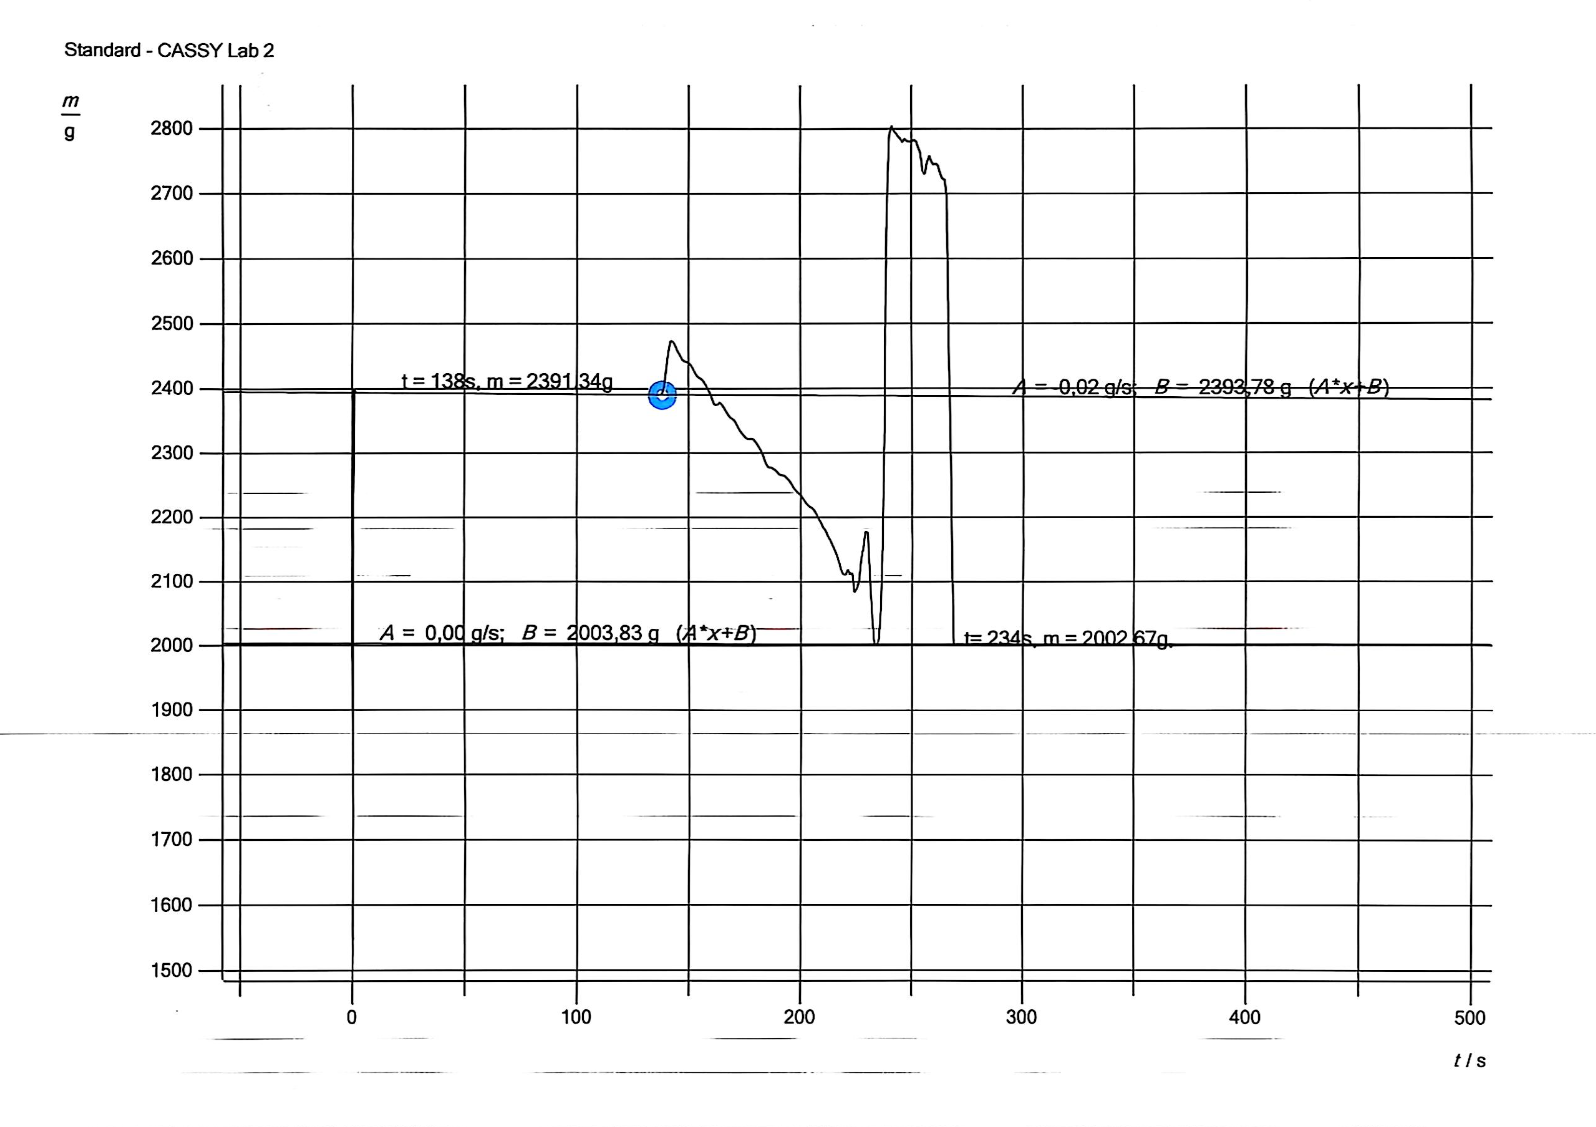
\includegraphics[width=0.8\textwidth]{Images/cassy.png}
    \caption{Mit CASSY aufgenommener zeitlicher Verlauf der Masse des
    Dewargefäßes mit flüssigem Stickstoff.}
    \label{fig:cassy_tv2}
\end{figure}
\noindent
Auch ohne das Einbringen des Aluminiumkörpers nimmt die Masse des flüssigen
Stickstoffs durch die kontinuierliche Verdampfung mit der Zeit ab. Diese
Hintergrundverdampfung muss von der während des Abkühlvorgangs beobachteten
Massenabnahme abgezogen werden.
\noindent
Aus den linearen Bereichen des CASSY-Diagramms wurden Verdampfungsraten von
näherungsweise

\begin{equation}
0{,}02\,\mathrm{\frac{g}{s}}
\end{equation}
\noindent
beziehungsweise

\begin{equation}
0{,}00\,\mathrm{\frac{g}{s}}
\end{equation}
\noindent
erhalten. Eine tatsächlich vollständig verschwindende Verdampfungsrate ist für
flüssigen Stickstoff unter den Versuchsbedingungen nicht realistisch. Daher wird
für die weitere Auswertung der Betrag

\begin{equation}
\boxed{
\left|\dot m_\mathrm{N_2}\right|
=
0{,}02\,\mathrm{\frac{g}{s}}
}
\end{equation}
\noindent
als realistische natürliche Verdampfungsrate verwendet.
\noindent
Die unterschiedliche Bestimmung der Verdampfungsrate vor und nach dem eigentlichen
Abkühlvorgang zeigt bereits, dass diese Korrektur nur näherungsweise möglich ist.


\subsubsection{Korrektur der verdampften Stickstoffmasse}
\noindent
Aus dem CASSY-Diagramm wurden unmittelbar vor beziehungsweise nach dem
Abkühlvorgang die Werte

\begin{equation}
t_1=138\,\mathrm{s},
\qquad
m_1=2391{,}34\,\mathrm{g}
\end{equation}
\noindent
und

\begin{equation}
t_2=234\,\mathrm{s},
\qquad
m_2=2002{,}67\,\mathrm{g}
\end{equation}
\noindent
abgelesen.
\noindent
Damit beträgt die gesamte beobachtete Massenabnahme

\begin{align}
\Delta m
&=
m_1-m_2\\
&=
2391{,}34\,\mathrm{g}
-
2002{,}67\,\mathrm{g}\\
&=
388{,}67\,\mathrm{g}.
\end{align}
\noindent
Das betrachtete Zeitintervall beträgt

\begin{align}
\Delta t
&=
t_2-t_1\\
&=
234\,\mathrm{s}-138\,\mathrm{s}\\
&=
96\,\mathrm{s}.
\end{align}
\noindent
Während dieses Zeitraums wäre aufgrund der natürlichen Verdampfung auch ohne den
Aluminiumkörper eine Stickstoffmasse von

\begin{align}
m_\mathrm{H}
&=
\left|\dot m_\mathrm{N_2}\right|\Delta t\\
&=
0{,}02\,\mathrm{\frac{g}{s}}
\cdot96\,\mathrm{s}\\
&=
1{,}92\,\mathrm{g}
\end{align}
\noindent
verdampft.
\noindent
Die tatsächlich durch das Abkühlen des Aluminiumkörpers verursachte
Stickstoffverdampfung beträgt daher

\begin{align}
m_\mathrm{V}
&=
\Delta m-m_\mathrm{H}\\
&=
388{,}67\,\mathrm{g}
-
1{,}92\,\mathrm{g}\\
&=
386{,}75\,\mathrm{g}.
\end{align}
\noindent
Damit ergibt sich

\begin{equation}
\boxed{
m_\mathrm{V}=386{,}75\,\mathrm{g}
}.
\end{equation}


\subsubsection{Bestimmung der spezifischen Wärmekapazität über die Verdampfungswärme}
\noindent
Die beim Abkühlen des Aluminiumkörpers abgegebene Wärmeenergie führt zur
Verdampfung des flüssigen Stickstoffs. Es gilt daher

\begin{equation}
Q_\mathrm{V}m_\mathrm{V}
=
m_\mathrm{Al}c_\mathrm{Al}
\left(T_1-T_2\right),
\end{equation}
\noindent
wobei für die spezifische Verdampfungswärme des Stickstoffs

\begin{equation}
Q_\mathrm{V}
=
199\,\frac{\mathrm{J}}{\mathrm{g}}
\end{equation}
\noindent
verwendet wird.
\noindent
Die Temperatur des Aluminiumkörpers unmittelbar vor dem Eintauchen in den
flüssigen Stickstoff wurde während des Versuchs nicht protokolliert. Da sich der
Körper zuvor bei Raumtemperatur befand, wird diese für die Auswertung auf

\begin{equation}
\boxed{
T_1\approx24^\circ\mathrm{C}
}
\end{equation}
\noindent
geschätzt.
\noindent
Dieser Wert stellt ausdrücklich keinen gemessenen Wert dar und ist daher als
zusätzliche systematische Unsicherheit der Auswertung anzusehen.
\noindent
Nach dem vollständigen Abkühlen wird angenommen, dass der Aluminiumkörper die
Temperatur des flüssigen Stickstoffs angenommen hat:

\begin{equation}
T_2=-196^\circ\mathrm{C}.
\end{equation}
\noindent
Die Temperaturdifferenz beträgt somit

\begin{equation}
T_1-T_2
=
24^\circ\mathrm{C}-(-196^\circ\mathrm{C})
=
220\,\mathrm{K}.
\end{equation}
\noindent
Auflösen der Energiebilanz nach der spezifischen Wärmekapazität ergibt

\begin{equation}
c_\mathrm{Al,V}
=
\frac{
Q_\mathrm{V}m_\mathrm{V}
}{
m_\mathrm{Al}(T_1-T_2)
}.
\end{equation}
\noindent
Einsetzen ergibt

\begin{align}
c_\mathrm{Al,V}
&=
\frac{
199\,\frac{\mathrm{J}}{\mathrm{g}}
\cdot386{,}75\,\mathrm{g}
}{
488{,}03\,\mathrm{g}
\cdot220\,\mathrm{K}
}\\
&=
0{,}716827\ldots\,
\frac{\mathrm{J}}{\mathrm{g\,K}}.
\end{align}
\noindent
Da die Raumtemperatur von $24^\circ\mathrm{C}$ lediglich abgeschätzt und nicht
gemessen wurde, wäre die Angabe aller berechneten Nachkommastellen nicht
gerechtfertigt. Als Ergebnis wird daher

\begin{equation}
\boxed{
c_\mathrm{Al,V}
\approx
0{,}72\,\frac{\mathrm{J}}{\mathrm{g\,K}}
}
\end{equation}
\noindent
angegeben.


\subsubsection{Vergleich der beiden Methoden mit Teilversuch 1}
\noindent
In Teilversuch 1 wurde für Aluminium die spezifische Wärmekapazität

\begin{equation}
c_\mathrm{Al,TV1}
=
0{,}72187\,\frac{\mathrm{J}}{\mathrm{g\,K}}
\end{equation}
\noindent
bestimmt.
\noindent
Damit ergibt sich folgende Übersicht:

\begin{table}[htbp]
    \centering
    \caption{Vergleich der bestimmten spezifischen Wärmekapazitäten von Aluminium.}
    \label{tab:vergleich_tv2}
    \begin{tabular}{l|c}
        \hline
        Methode &
        $c_\mathrm{Al}$ in $\mathrm{J/(g\,K)}$\\
        \hline
        Teilversuch 2: Kalorimeter
        & $0{,}698$\\
        Teilversuch 2: Verdampfungswärme
        & $0{,}72$\\
        Teilversuch 1: Kalorimeter
        & $0{,}72187$\\
        \hline
    \end{tabular}
\end{table}
\noindent
Unter Verwendung der ungerundeten Rechenwerte beträgt die relative Abweichung
der Kalorimetermethode aus Teilversuch 2 vom Ergebnis aus Teilversuch 1

\begin{align}
\delta_\mathrm{Kal}
&=
\frac{
c_\mathrm{Al,Kal}-c_\mathrm{Al,TV1}
}{
c_\mathrm{Al,TV1}
}
\cdot100\,\%\\
&=
\frac{
0{,}698279-0{,}72187
}{
0{,}72187
}
\cdot100\,\%\\
&\approx
-3{,}3\,\%.
\end{align}
\noindent
Für die Methode über die Verdampfungswärme ergibt sich entsprechend

\begin{align}
\delta_\mathrm{V}
&=
\frac{
0{,}716827-0{,}72187
}{
0{,}72187
}
\cdot100\,\%\\
&\approx
-0{,}7\,\%.
\end{align}
\noindent
Die beiden in Teilversuch 2 erhaltenen Werte unterscheiden sich untereinander
um etwa $2{,}6\,\%$ und liegen beide unterhalb des in Teilversuch 1 bestimmten
Wertes.


\subsubsection{Interpretation der Temperaturabhängigkeit}
\noindent
Nach der klassischen Regel von Dulong und Petit sollte die molare Wärmekapazität
eines Festkörpers für hinreichend hohe Temperaturen näherungsweise konstant sein.
Bei tiefen Temperaturen versagt diese Näherung jedoch.
\noindent
Die Gitterschwingungen eines Festkörpers besitzen quantisierte Energien. Bei
niedrigen Temperaturen steht nicht genügend thermische Energie zur Verfügung,
um alle möglichen Schwingungszustände anzuregen. Die Wärmekapazität nimmt daher
mit sinkender Temperatur ab.
\noindent
In Teilversuch 1 wurde die mittlere Wärmekapazität von Aluminium in einem
vergleichsweise hohen Temperaturbereich bestimmt. In Teilversuch 2 umfasst das
betrachtete Temperaturintervall dagegen Temperaturen bis hinunter zur
Siedetemperatur von flüssigem Stickstoff. Daher wird für Teilversuch 2 ein
niedrigerer Mittelwert der Wärmekapazität erwartet.
\noindent
Beide in Teilversuch 2 bestimmten Werte liegen tatsächlich unterhalb des
Ergebnisses aus Teilversuch 1. Die Abnahme ist jedoch insbesondere bei der
Methode über die Verdampfungswärme nur gering. Aufgrund der vorhandenen
systematischen Unsicherheiten ist daher vor allem die qualitative Tendenz
aussagekräftig. Die Messergebnisse sind mit der erwarteten Abnahme der
Wärmekapazität bei tiefen Temperaturen vereinbar.


\subsubsection{Diskussion der systematischen Unsicherheiten}
\noindent
Die größten Unsicherheiten des Versuchs liegen nicht in den Wägungen selbst,
sondern in den experimentellen Randbedingungen.
\noindent
Bei der Bestimmung über die Verdampfungswärme stellt insbesondere die
Anfangstemperatur des Aluminiumkörpers eine Unsicherheit dar. Sie wurde nicht
gemessen, sondern nachträglich mit etwa $24^\circ\mathrm{C}$ abgeschätzt.
Da die Wärmekapazität über die Temperaturdifferenz

\begin{equation}
T_1-T_2
\end{equation}
\noindent
bestimmt wird, wirkt sich eine Abweichung der tatsächlichen Raumtemperatur direkt
auf das Ergebnis aus. Beispielsweise würde bereits eine Änderung der angenommenen
Raumtemperatur um einige Kelvin das Ergebnis merklich verändern.
\noindent
Eine weitere Unsicherheit entsteht durch die Bestimmung der natürlichen
Verdampfungsrate des Stickstoffs. Aus dem CASSY-Diagramm wurden unterschiedliche
Steigungen erhalten. Der Wert von $0{,}00\,\mathrm{g/s}$ kann aufgrund der
begrenzten Auflösung der angegebenen Fitparameter nicht als tatsächlich
verschwindende Verdampfung interpretiert werden. Die Wahl von
$0{,}02\,\mathrm{g/s}$ stellt daher eine begründete Näherung dar.
\noindent
Während des Eintauchens des Aluminiumkörpers kommt es außerdem zu starkem Sieden
des Stickstoffs. Bewegungen des Dewargefäßes, mechanische Einflüsse auf die Waage,
Spritzer oder verdampfende Stickstofftröpfchen können den gemessenen Masseverlauf
beeinflussen.
\noindent
Für beide Methoden wird angenommen, dass der Aluminiumkörper im flüssigen
Stickstoff tatsächlich die Temperatur von $-196^\circ\mathrm{C}$ erreicht.
Ist der Körper noch nicht vollständig thermisch ausgeglichen, stimmt die
verwendete Temperaturdifferenz nicht exakt mit der tatsächlichen überein.
\noindent
Bei der Kalorimetermethode kann sich der Aluminiumkörper zudem bereits während
des Transfers vom flüssigen Stickstoff zum Kalorimeter erwärmen. Seine tatsächliche
Temperatur beim Eintauchen in das Wasser wäre dann höher als die angenommenen
$-196^\circ\mathrm{C}$. Da in der Rechnung dadurch eine zu große
Temperaturdifferenz verwendet wird, würde die spezifische Wärmekapazität
tendenziell zu klein bestimmt. Dies kann zumindest teilweise erklären, warum mit
der Kalorimetermethode der niedrigste Wert erhalten wurde.
\noindent
Zusätzlich können am Aluminiumkörper anhaftende Reste von flüssigem Stickstoff
in das Kalorimeter gelangen und dort verdampfen. Die dafür benötigte
Verdampfungswärme wird dem Kalorimeter entzogen, obwohl sie in der einfachen
Energiebilanz nicht separat berücksichtigt wird.
\noindent
Auch das Kalorimeter ist nicht vollkommen wärmeisoliert. Da die Temperatur des
Kalorimeterwassers während des Versuchs von etwa $38^\circ\mathrm{C}$ auf etwa
$18^\circ\mathrm{C}$ fällt und damit den Bereich der Raumtemperatur durchläuft,
ändert sich während des Vorgangs zusätzlich die Richtung des Wärmeaustausches mit
der Umgebung. Dies kann die beobachtete Ausgleichstemperatur beeinflussen.
\noindent
Eine formale Fehlerfortpflanzung wird für diesen Teilversuch nicht durchgeführt.
Die genannten systematischen Effekte sind jedoch deutlich größer als die reine
Auflösung der verwendeten Waage und bestimmen daher wesentlich die tatsächliche
Genauigkeit der Ergebnisse.


\subsubsection{Ergebnis}
\noindent
Mit der Kalorimetermethode wurde für die mittlere spezifische Wärmekapazität von
Aluminium im untersuchten tiefen Temperaturbereich

\begin{equation}
\boxed{
c_\mathrm{Al,Kal}
=
0{,}698\,\frac{\mathrm{J}}{\mathrm{g\,K}}
}
\end{equation}
\noindent
bestimmt.
\noindent
Die unabhängige Bestimmung über die beim Abkühlen verdampfte Stickstoffmenge
ergab

\begin{equation}
\boxed{
c_\mathrm{Al,V}
\approx
0{,}72\,\frac{\mathrm{J}}{\mathrm{g\,K}}
}.
\end{equation}
\noindent
Zum Vergleich wurde in Teilversuch 1

\begin{equation}
c_\mathrm{Al,TV1}
=
0{,}72187\,\frac{\mathrm{J}}{\mathrm{g\,K}}
\end{equation}
\noindent
bestimmt.
\noindent
Die Ergebnisse aus Teilversuch 2 liegen damit um etwa $3{,}3\,\%$
beziehungsweise $0{,}7\,\%$ unter dem Ergebnis aus Teilversuch 1. Die Richtung
der Abweichung entspricht der theoretisch erwarteten Abnahme der
Wärmekapazität von Aluminium bei tiefen Temperaturen. Aufgrund der teilweise
nur abgeschätzten experimentellen Größen und der Unsicherheit der
Verdampfungskorrektur ist der quantitative Unterschied jedoch mit einer
größeren systematischen Unsicherheit behaftet.


\newpage
\section{Teilversuch III: Gefriervorgang von reinem Wasser}
In Teilversuch III wurde destilliertes Wasser in einem Salz-Eiswasserbad mit einer Temperatur von ca. $\qty{-6}{\degreeCelsius}$ gekühlt. Hierbei konnte folgender 
Temperaturverlauf beobachtet werden:
\begin{figure}[H]
    \centering
    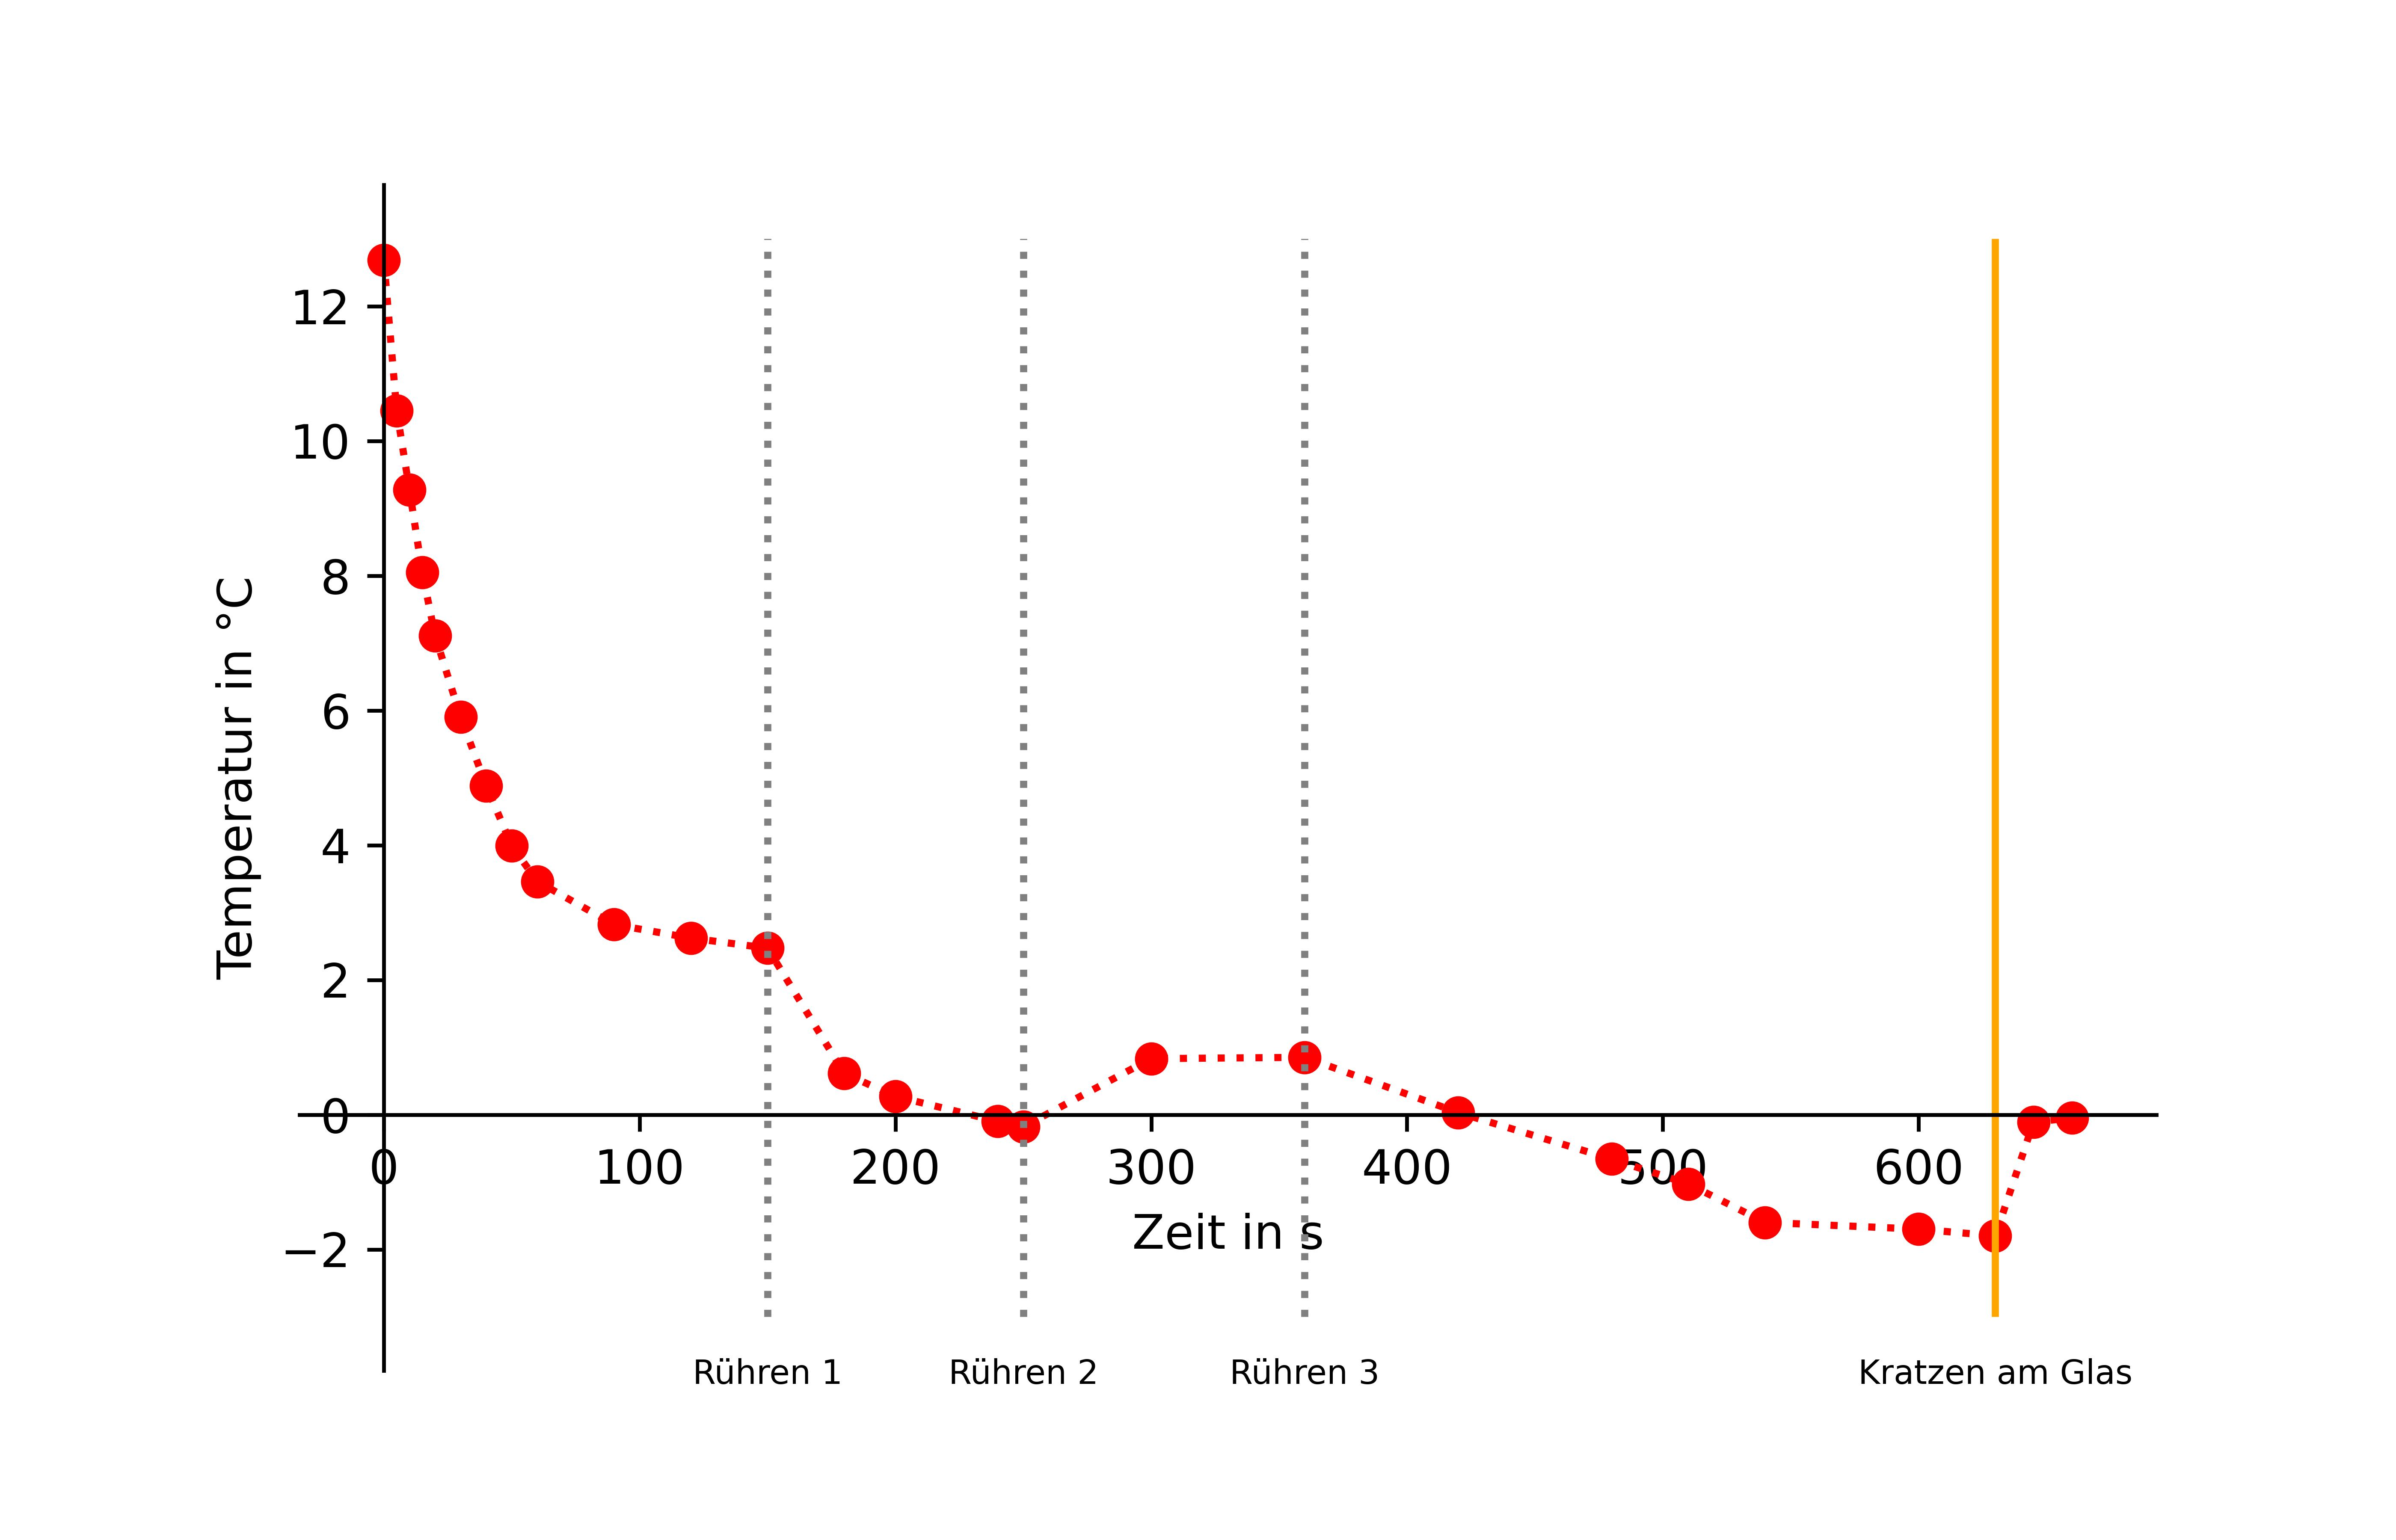
\includegraphics[width=1\textwidth]{./Images/TV3_TempVerlaufDiag.jpg}
    \caption{Temperaturverlauf des destillierten Wassers}
    \label{fig:TempVerlaufDiag}
\end{figure}
\noindent
Es ist erkennbar, dass die Temperatur zunächst absinkt und dann bei etwa $\qty{2}{\degreeCelsius}$ zu stagnieren scheint. Nach dem ersten Rühren sinkt die Temperatur dannn 
allerdings weiter. Dies liegt daran, dass durch das Rühren Konvektion auftreten kann und so kaltes Wasser vom Rand des Reagenzglases auch in die Mitte zum Temperaturfühler gelangt.
Interessanterweise steigt allerdings die Temperatur beim erneuten durchmischen wieder an (auf ca. $\qty{1}{\degreeCelsius}$). Dieses Phänomen hat keine direkte physikalische Erklärung und ist höchstwahrscheinlich 
auf eine ungünstige Positionierung des Thermometers (evtl mit Kontakt zur Wand des Reagenzglases) zurückzuführen. Nach dem dritten Rühren setzt sich der Abkühlungsverlauf wieder wie zuvor fort. 
Hierbei wird eine minimale Temperatur von ca. $\qty{-1.8}{\degreeCelsius}$ erreicht. Dies ist überraschend, da das Wasser bei dieser Temperatur immer noch flüssig ist, obwohl die 
Temperatur unterhalb des Schmelzpunktes von Wasser liegt. Erklärt werden kann dies dadurch, dass sich aufgrund der extremen reinheit des destillierten Wassers kein 
Kristallisationskeim im Wasser befindet, weshalb keine Eiskristalle gebildet werden können. 
Durch das Kratzen an der Reagenzglaswand entstehen durch Abrieb kleine Partikel, die als Kristallisationskeime wirken. Dadurch können sich nun Eiskristalle bilden und 
das Wasser gefriert schlagartig. Da bei diesem Phasenübergang Wärme freigesetzt wird, steigt die Temperatur schnell auf einen Wert von ca. $\qty{0}{\degreeCelsius}$. 
Bei dieser Temperatur stabilisiert sich die Temperatur, da bei höheren Temperaturen keine weiteren Eiskristalle mehr gebildet werden.
\newpage
\section{Teilversuch IV: Dampfdruckkurve von Wasser}
\subsection{Auswertung der Dampfdruckkurve}
In Teilversuch IV wurde die Dampfdruckkurve von Wasser aufgezeichnet. Hierzu wurde folgende Apparatur verwendet:
\begin{figure}[H]
    \centering
    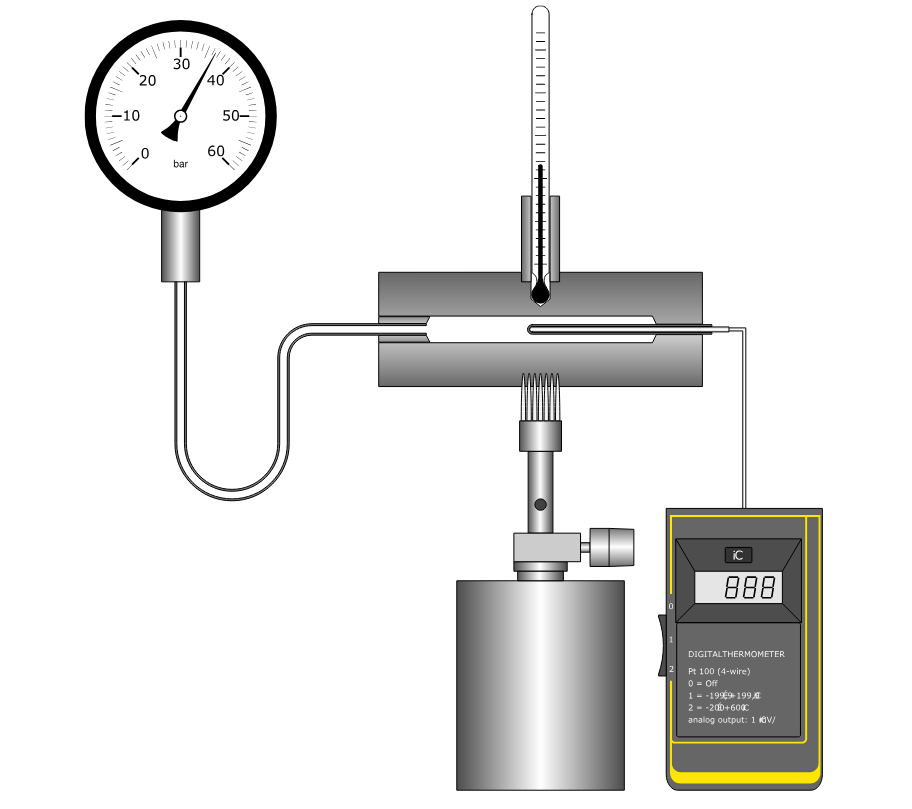
\includegraphics[width=0.5\textwidth]{./Images/DampfdruckApparat.png}
    \source{Abb. 11 Versuchsanleitung APW - P2-Praktikum}
    \caption{Versuchsaufbau zur Bestimmung der Dampfdruckkurve}
    \label{fig:DampfdruckApparat}
\end{figure}
\noindent
Mit dieser wurden mehrere Temperatur-Druck-Wertepaare gemessen.
Plottet man diese und fittet eine Exponentialfunktion, erhält man folgenden Graphen:
(Hierbei wurde zu den jeweiligen Manometerwerten noch ein Atmosphärendruck von $p_{\mathrm{atm}}\qty{0.965}{bar}$ addiert)
\begin{figure}[H]
    \centering
    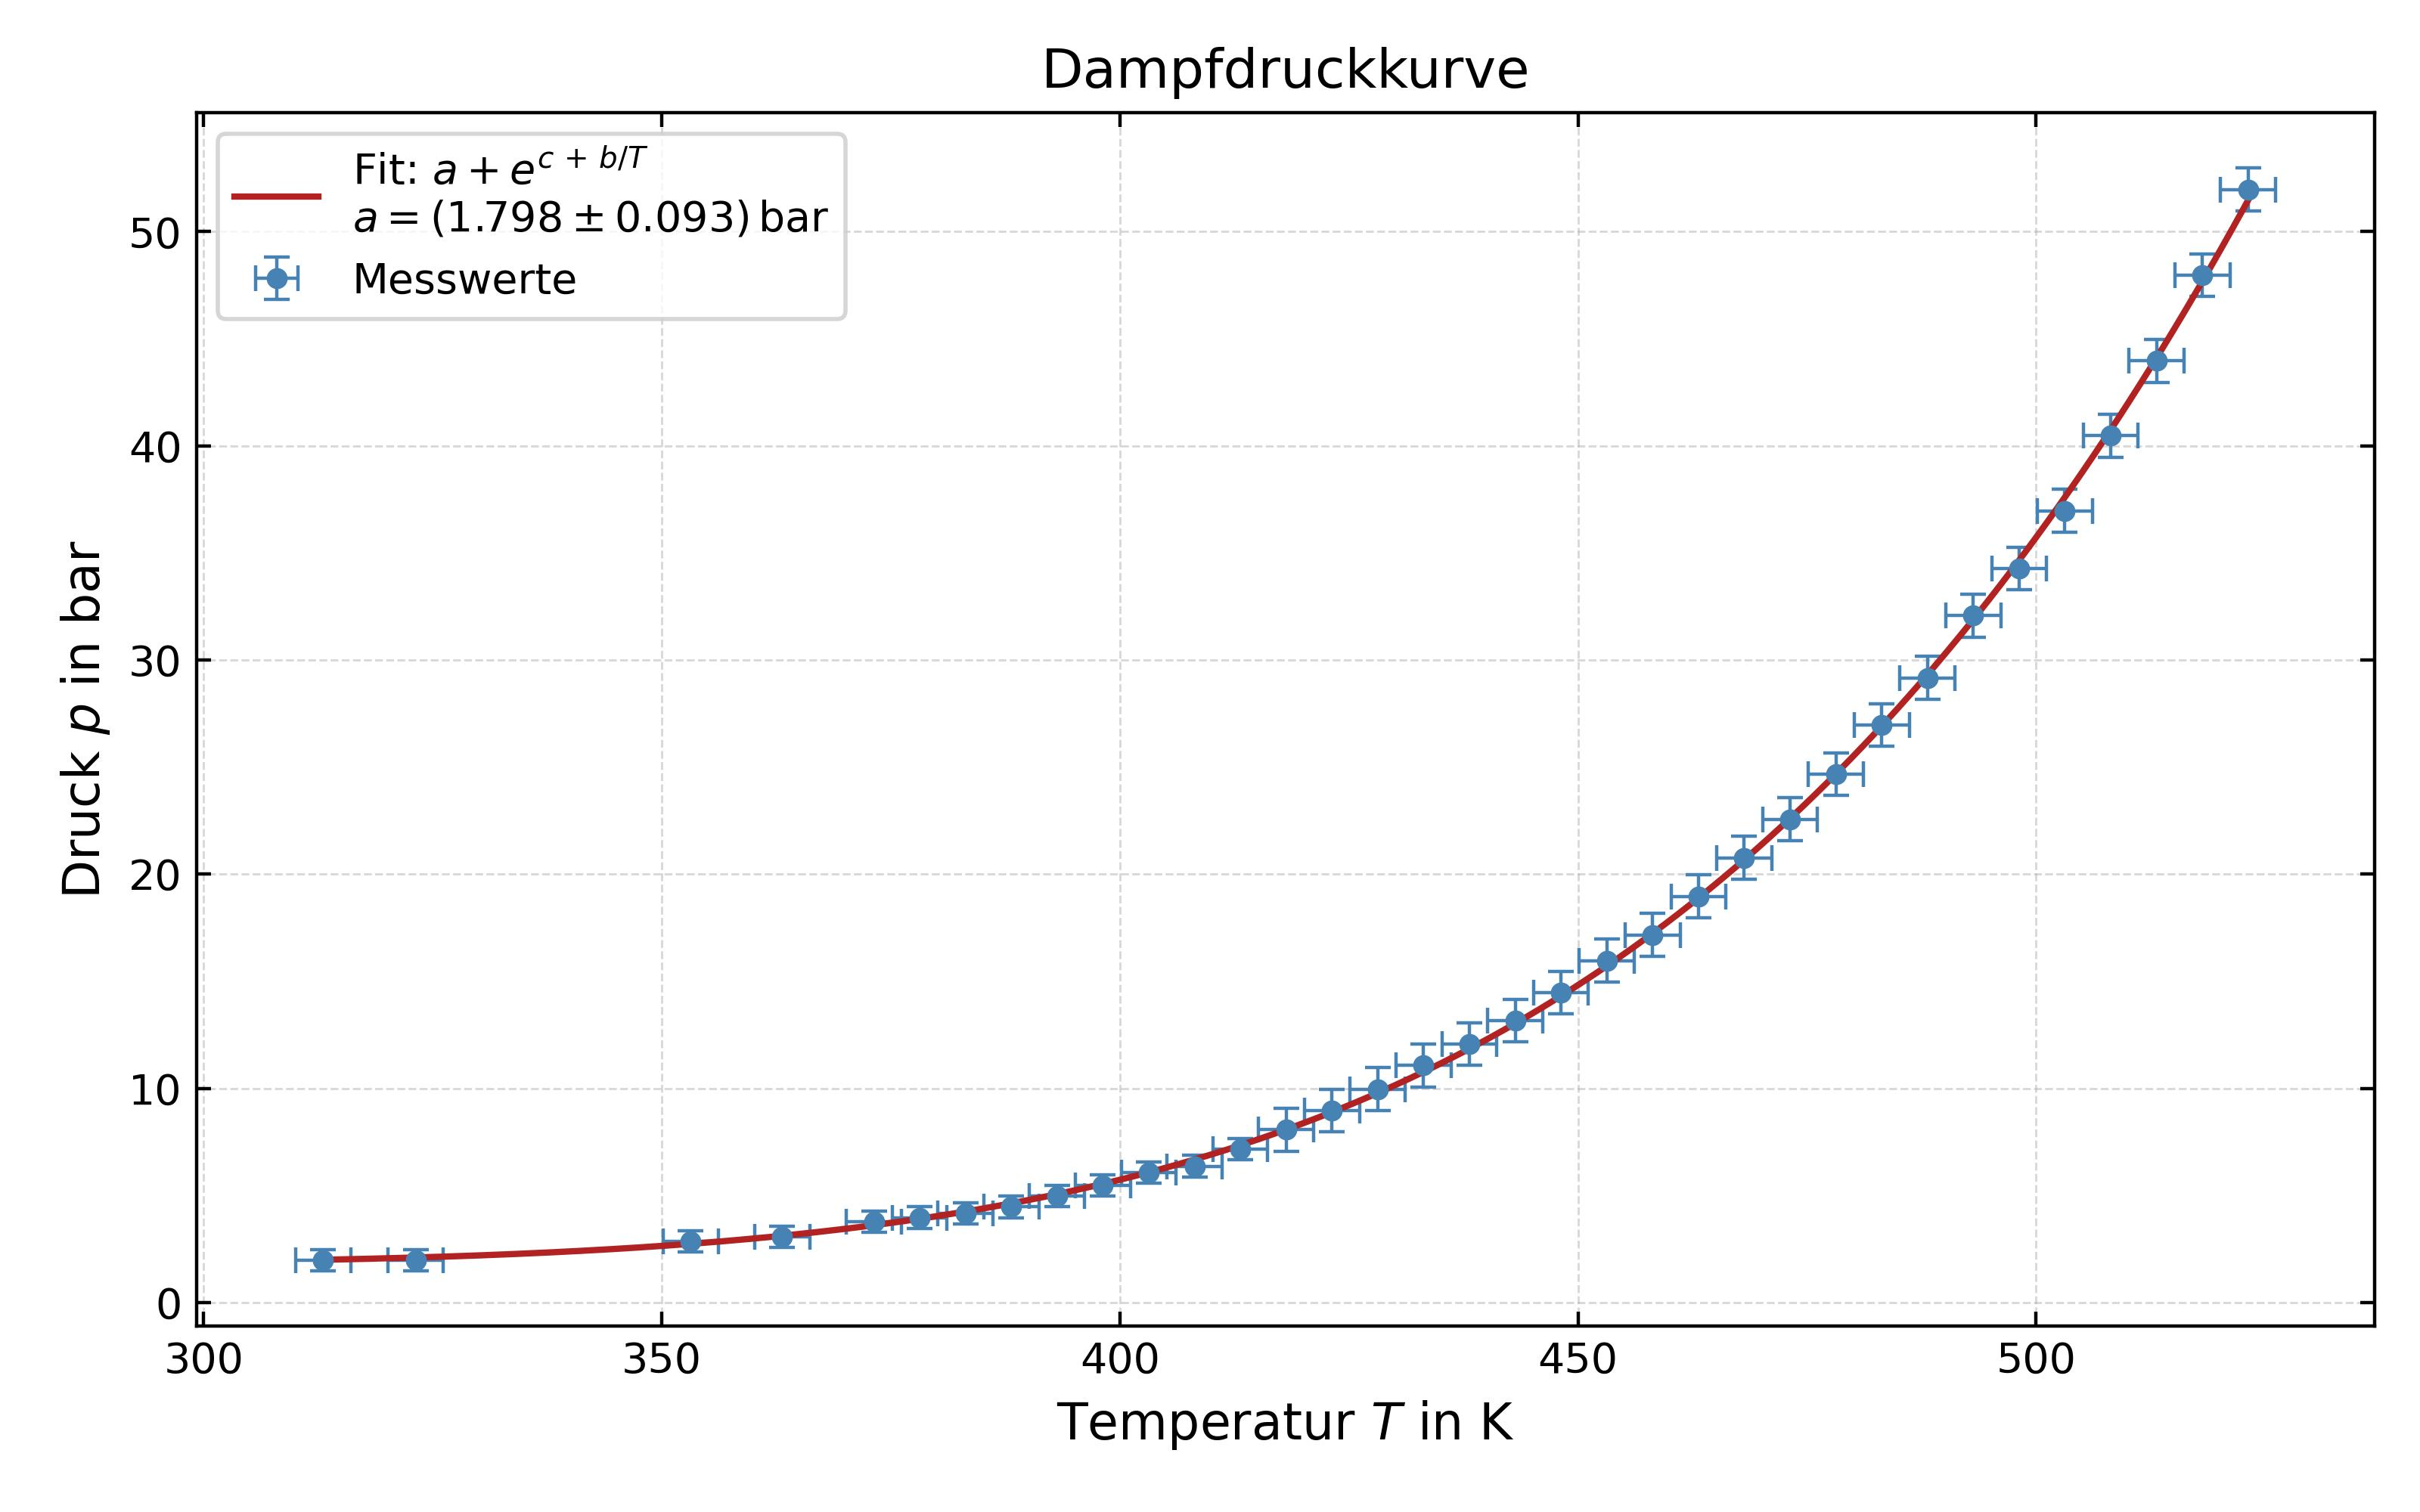
\includegraphics[width=.7\textwidth]{./Images/PTDiagramm.jpg}
    \caption{Gemessenes $p(T)$-Diagramm}
    \label{fig:PTDiagramm}
\end{figure}
\noindent
Folgt man diesem Graphen, läge der Druck bei $T = \qty{0}{K}$ bei $a = (1.798 \pm 0.093) \si{bar}$. Allerdings ist bekannt, dass der Dampfdruck von Wasser am absoluten 
Nullpunkt bei $\qty{0}{bar}$ liegen müsst, da die Teilchen hier keine Kinetische Energie haben. Das heißt, dass die gemessenen Werte einen zusätzlichen Partialdruck 
enthalten, der nicht auf den Dampfdruck des Wassers zurückzuführen ist. Dieser entsteht eventuell durch weiteres Gas, das zusätzlich zum Wasser im Aufbau eingeschlossen wurde und 
muss für die weitere Auswertung abgezogen werden.
Berücksichtigt man dies kann man nun $\ln(p)$ gegen $-\frac{1}{T}$ auftragen.
Die Fehler ergeben sich hierfür als:
\begin{equation}
    \begin{split}
        \Delta \ln(p)   &= \left(\frac{\partial}{\partial p} \ln(p)\right) \cdot \Delta p \\
                        &= \frac{\Delta p}{p}
    \end{split}
\end{equation}
und
\begin{equation}
    \begin{split}
        \Delta \left(-\frac{1}{T}\right)  &= \left(\frac{\partial}{\partial T} \frac{1}{T}\right) \Delta T \\
                                                        &= \frac{\Delta T}{T^2}
    \end{split}
\end{equation}
Der Plot dieser Daten ergibt folgendes:
\begin{figure}[H]
    \centering
    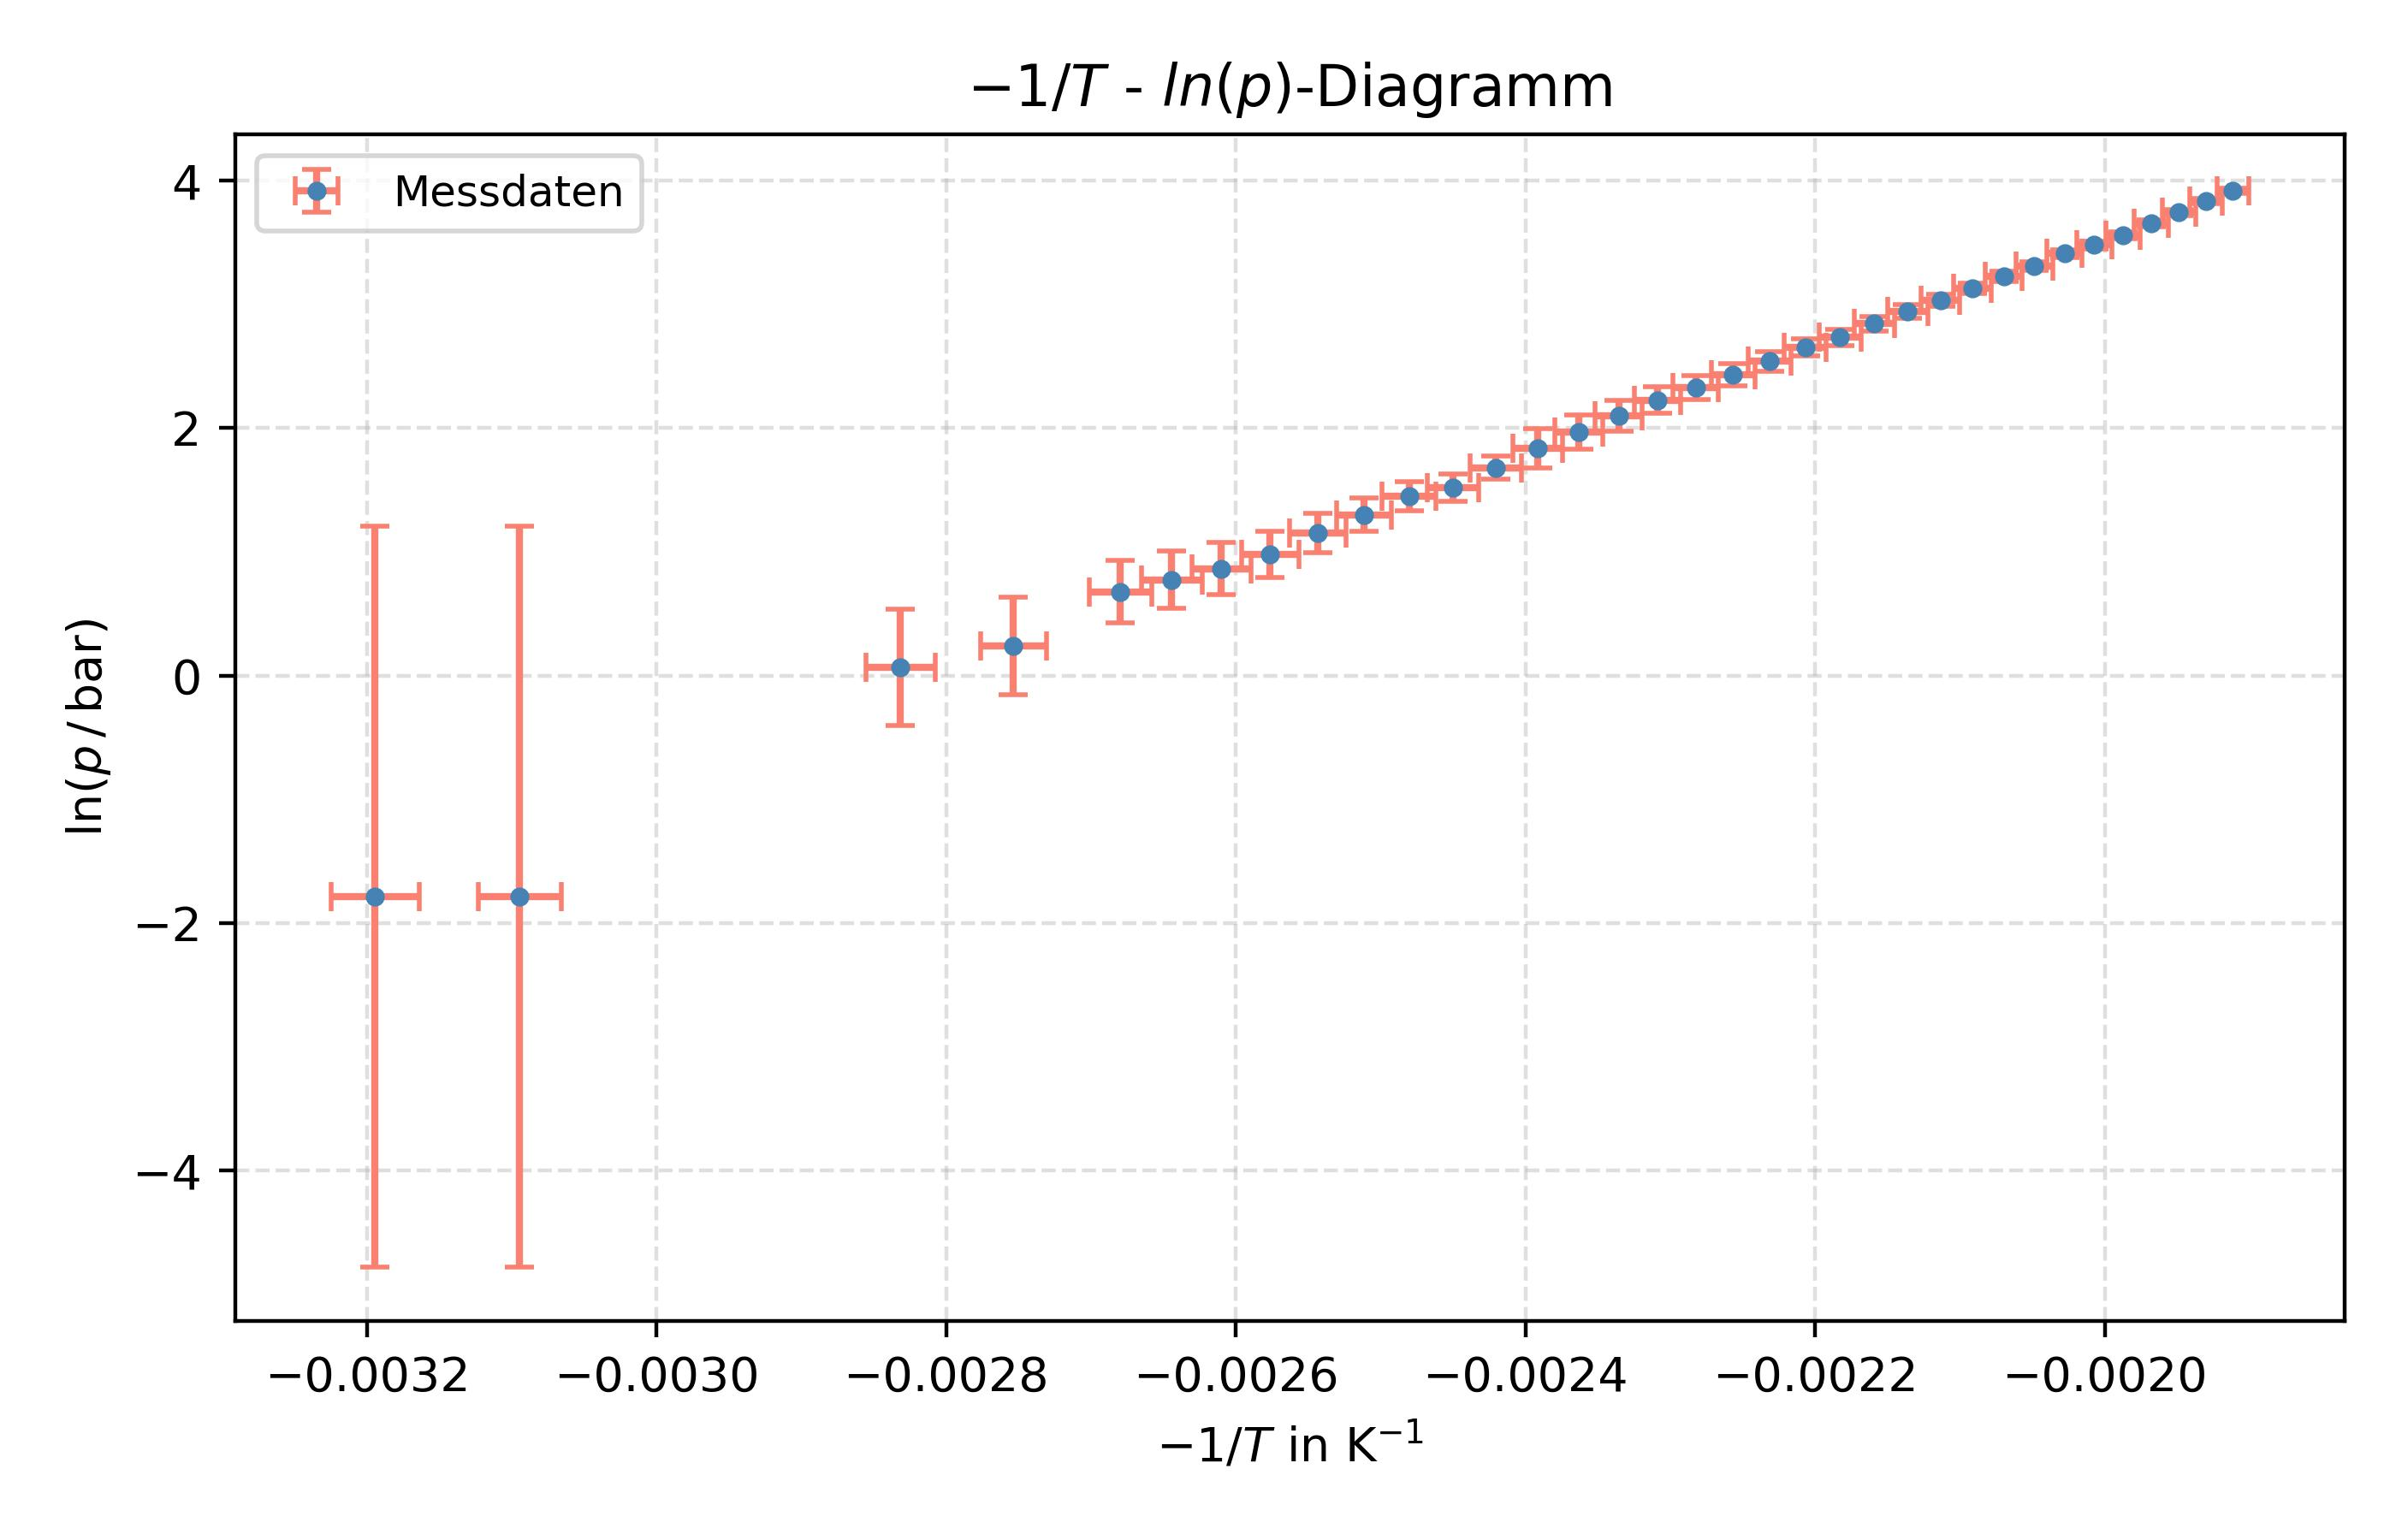
\includegraphics[width=1\textwidth]{./Images/TV4_lnPTDiagramm.jpg}
    \caption{$-1/T^2$-$\ln(p)$-Diagramm der Dampfdruckkurve}
    \label{fig:lnPTDiagramm}
\end{figure}
Es ist erkennbar, dass die Unsicherheiten der ersten beiden Messwerte extrem hoch sind. Sie liegen allerdings trotzdem innerhalb dieser Messunsicherheiten
auf der Geraden durch die anderen Punkte. Daher werden sie, um ein genaueres Ergebnis zu erhalten im folgenden vernachlässigt.
Mit dieser Vernachlässigung erhält man folgendes Diagramm:
\begin{figure}[H]
    \centering
    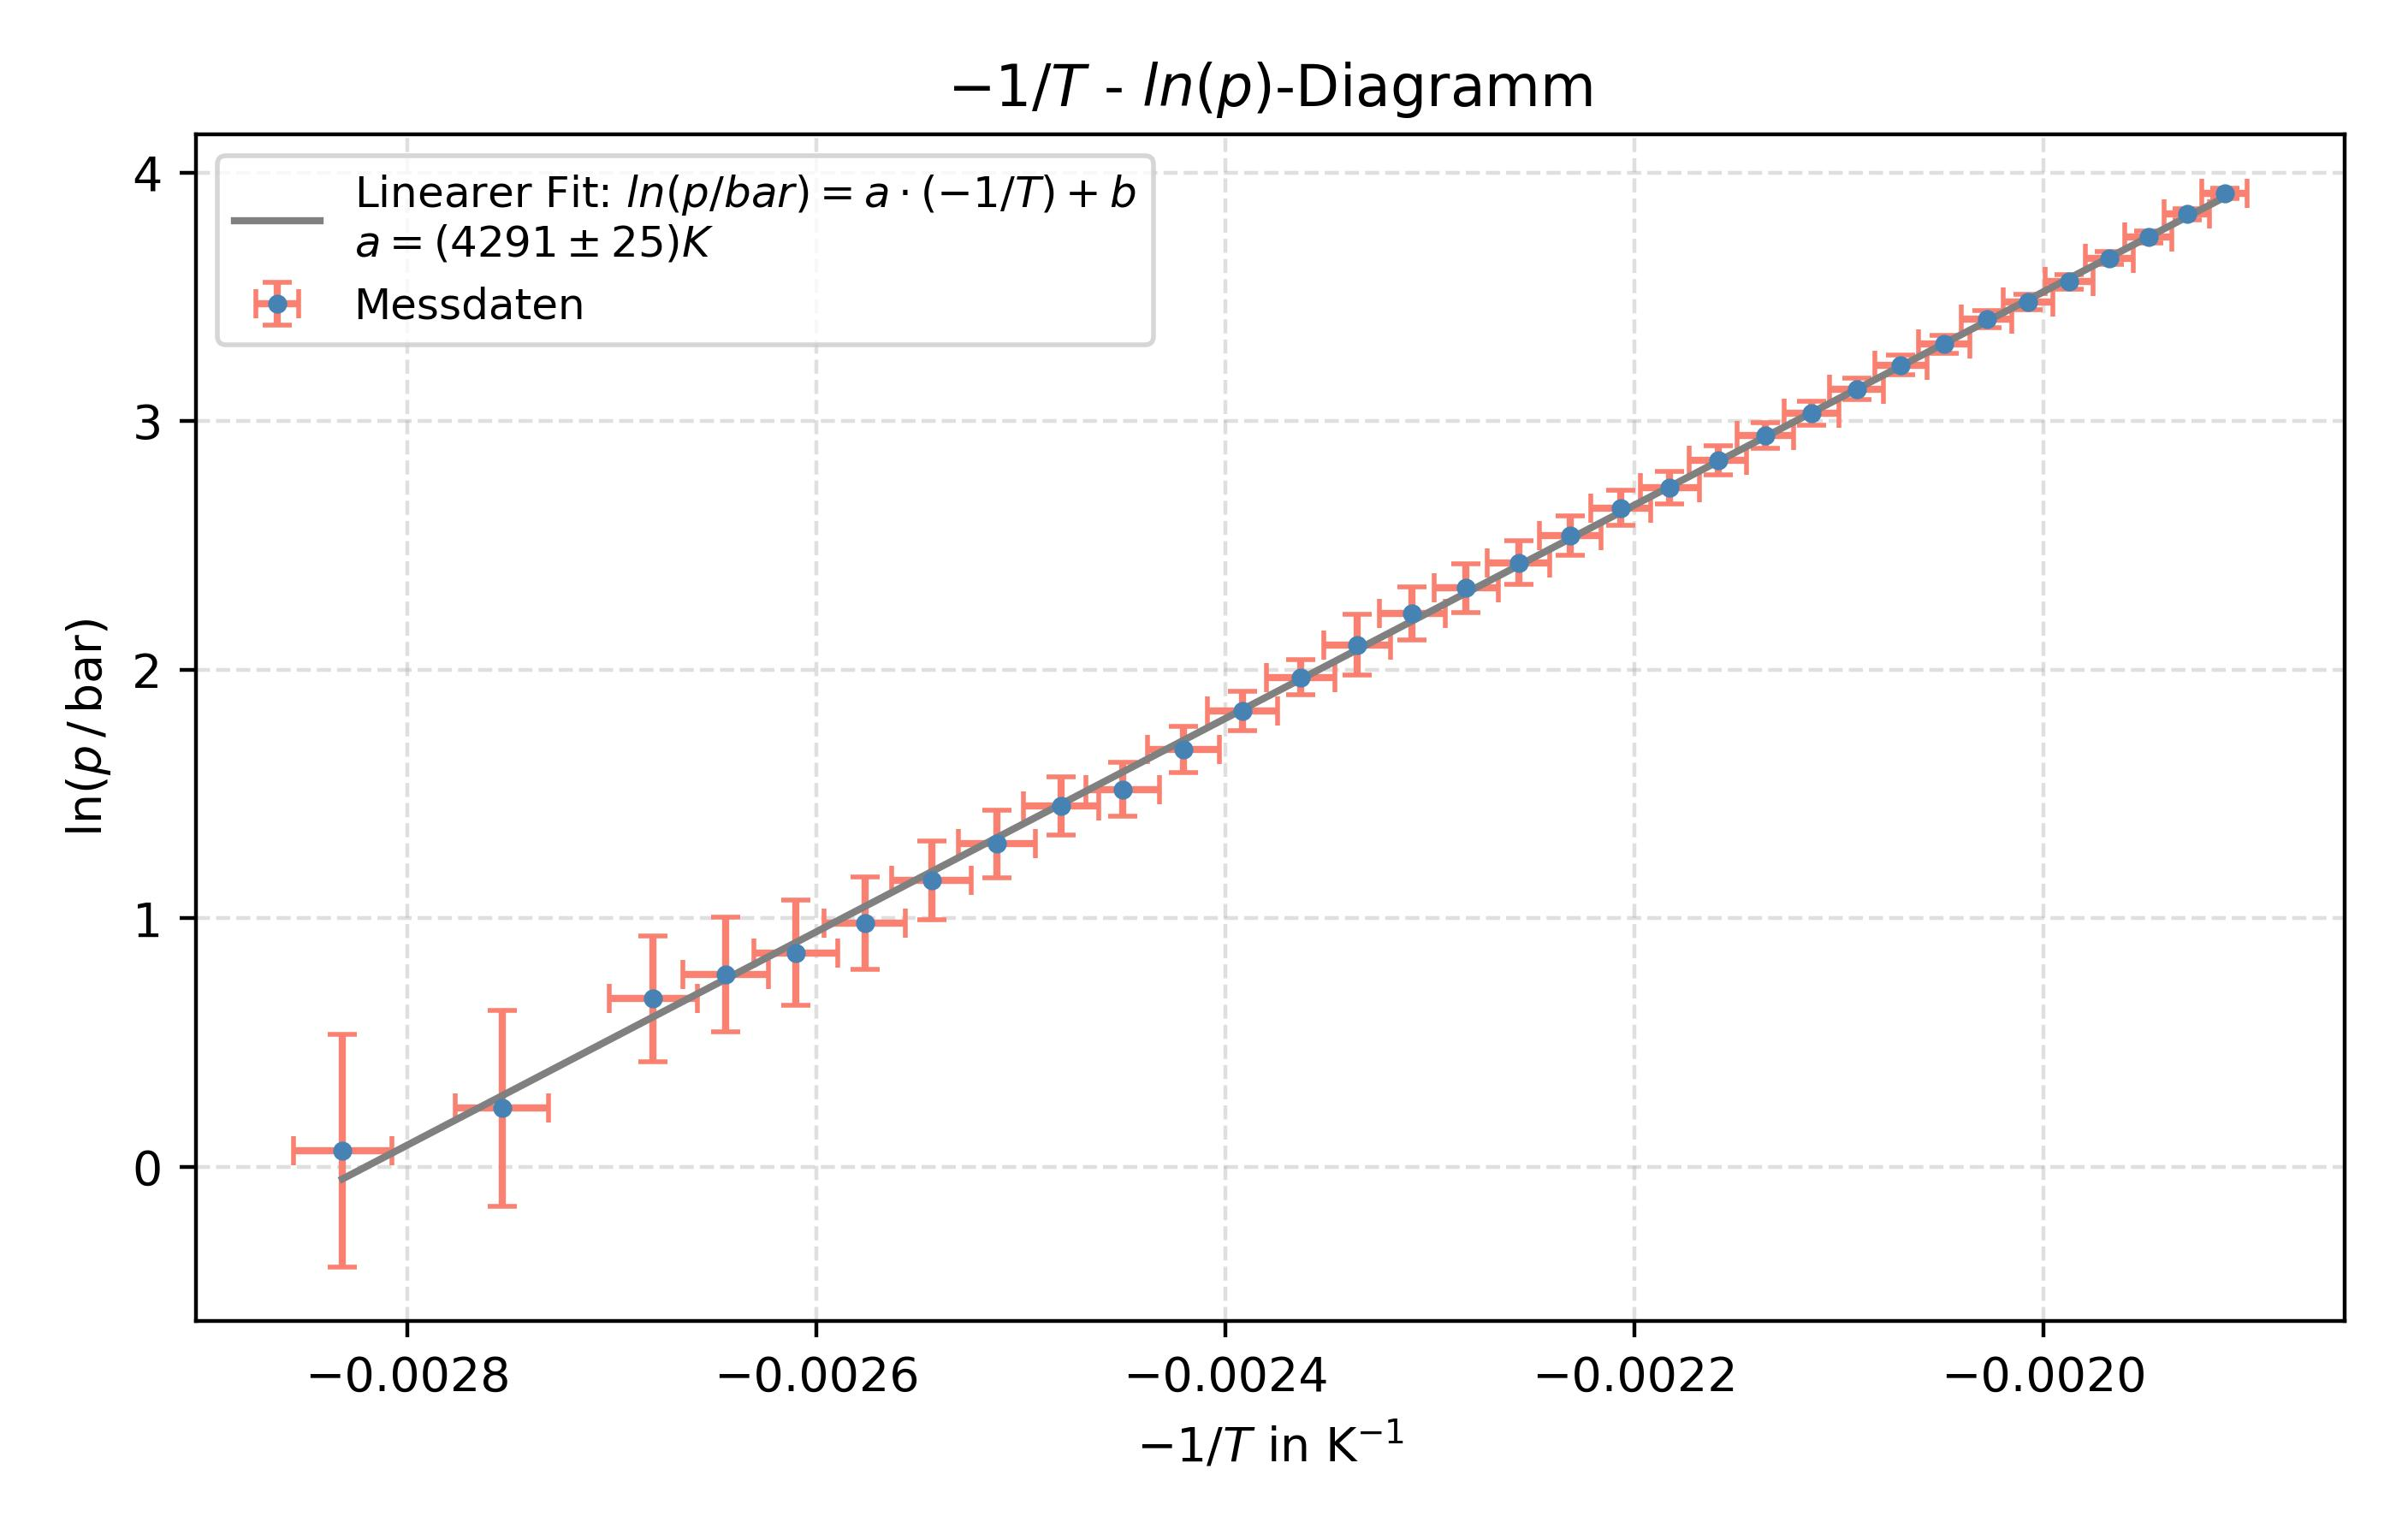
\includegraphics[width=1\textwidth]{./Images/TV4_lnPTDiagrammValsRemoved.jpg}
    \caption{$-1/T^2$-$\ln(p)$-Diagramm der Dampfdruckkurve ohne die ersten beiden Messwerte mit Ausgleichsgerade}
    \label{fig:lnPTDiagrammValsRemoved}
\end{figure}
\noindent
\subsection{Interpretation der Steigung}
Aus der Theorie gilt:
\begin{equation}
    \begin{split}
        p(T) = p_{\infty} \exp\left(-\frac{E_b}{k_B T}\right)
    \end{split}
\end{equation}
Wobei $E_b$ die Bindungsenergie der Teilchen in der Flüssigkeit ist.
Durch das Logarithmieren erhält man:
\begin{equation}
    \begin{split}
        \ln\left(\frac{p(T)}{\si{bar}}\right)   &= \ln \left(\frac{p_{\infty}}{\si{bar}}\right) + \frac{E_b}{k_B} \cdot \left(-\frac{1}{T}\right) \\
                                                &= a \cdot \left(-\frac{1}{T}\right) + b
    \end{split}
\end{equation}
Damit ergibt sich für die Bindungsenergie mithilfe der Steigung der Geraden:
\begin{equation}
    \begin{split}
        E_b &= k_B \cdot a \\
            &= (5.92 \pm 0.04) \times 10^{-20} \si{J}
    \end{split}
\end{equation}
Auf ein Mol bezogen ergibt sich:
\begin{equation}
    \begin{split}
        E_b^m   &= N_A E_b \\
                &= (35.68 \pm 0.21) \si{\kilo\joule \per \mol}
    \end{split}
\end{equation}  
Der Literaturwert liegt bei:
\begin{equation}
    E_{\mathrm{b, lit}}^m = 40.65 \si{\kilo\joule \per \mol}
\end{equation}
Dieser Wert liegt zwar in der Größenordnung des experimentell bestimmten Wertes, ist mit diesem allerdings im Rahmen der Messunsicherheiten nicht vereinbar.
Für diese Abweichung kann es verschiedene Gründe haben. 
Einerseits gilt die der Theorie zugrundeliegende Clausius-Clapeyron-Gleichung nur für ideale Gase. Allerings handelt es sich bei Wasserdampf, insbesondere 
Aufgrund der relativ starken intermolekularen Kräften nicht um ein ideales Gas. Zudem sind die Teilchenabstände bei den im Versuch auftretenden 
Drücken nicht mehr extrem groß, was ebenfalls den Annahmen über ein ideales Gas widerspricht. Dies könnte die Abweichung erklären. 
Zudem könnte auch die Hysterese des Thermometers ebenfalls zum Fehler beigetragen haben. Da die Temperatur im Versuch sehr schnell angestiegen ist, kann dieser Effekt 
nicht vernachlässigt werden.

\newpage
\section{Teilversuch V: Strahlung eines Hohlraumstrahlers}
\subsection{Theoretischer Hintergrund}
In Teilversuch V wurde die Strahlung eines Hohlraumstrahlers gemessen. Hierzu wurde ein Kalibrator zur Kalibrierung von Infrarotthermometern als schwarzer Strahler verwendet. 
Dann wurde die Intensität der Strahlung mithilfe einer Thermosäule gemessen. Diese gibt eine zur Intensität proportionale Spannung aus.
Ziel war es, das Stefan Boltzmann-Gesetz experimentell zu überprüfen.
Dieses besagt, dass die Strahlungsleistung eines Körpers Proportional zu $T_k^4$ ist:
\begin{equation}
    P = \sigma A T^4
\end{equation}
Im Versuch wurde eine zur Leistung proportionale Spannung aufgezeichnet. Diese Spannung wurde für die Umgebungstemperatur auf Null gesetzt. Es wurde also nur die 
Strahlung des Körpers gemessen, welche oberhalb der Leistung der Umgebungsstrahlung liegt. Damit liegt die gemessene Leistung bei:
\begin{equation}
    \begin{split}
        P_{\mathrm{eff}}    &= P_{\mathrm{kal}} - P_{\mathrm{umg}} \\
                            &= \sigma A (T^4 - T_0^4)
    \end{split}
\end{equation}
Es sollte also folgende Proportionalität nachgewiesen werden:
\begin{equation}
    U_{\mathrm{mess}} \propto (T^4 - T_0^4)
\end{equation}
Hierzu werden die gemessenen Werte inklusiv Unsicherheit der Spannungsmessung ($\Delta U = 0.04\%U + \qty{1}{\micro \volt}$) mithilfe eines Python-Scripts geplottet. Außerdem wurden eine optimale Gerade und ein Fehlerstreifen hindurchgelegt(Siehe Abb. \ref{fig:StefanBoltzmann})
Es ist erkennbar, dass tatsächlich alle Werte sehr nah an der Ausgleichsgerade liegen, was auf einen linearen Zusammenhang hindeutet. 
Außerdem hat die optimale Gerade einen Ordinatenabschnitt von $(-0.21 \pm 2.0) \si{\micro \volt}$, damit handelt es sich bei dieser im Rahmen der Messunsicherheiten um eine Ursprungsgerade.
Somit wäre die Proportionalität gezeigt und damit das Stefan-Boltzmann-Gesetz bestätigt.
\newgeometry{left=0cm,right=0cm,top=0cm,bottom=0cm}
    \begin{landscape}
        \thispagestyle{empty}
        \noindent
        \begin{figure}[H]
            \centering
            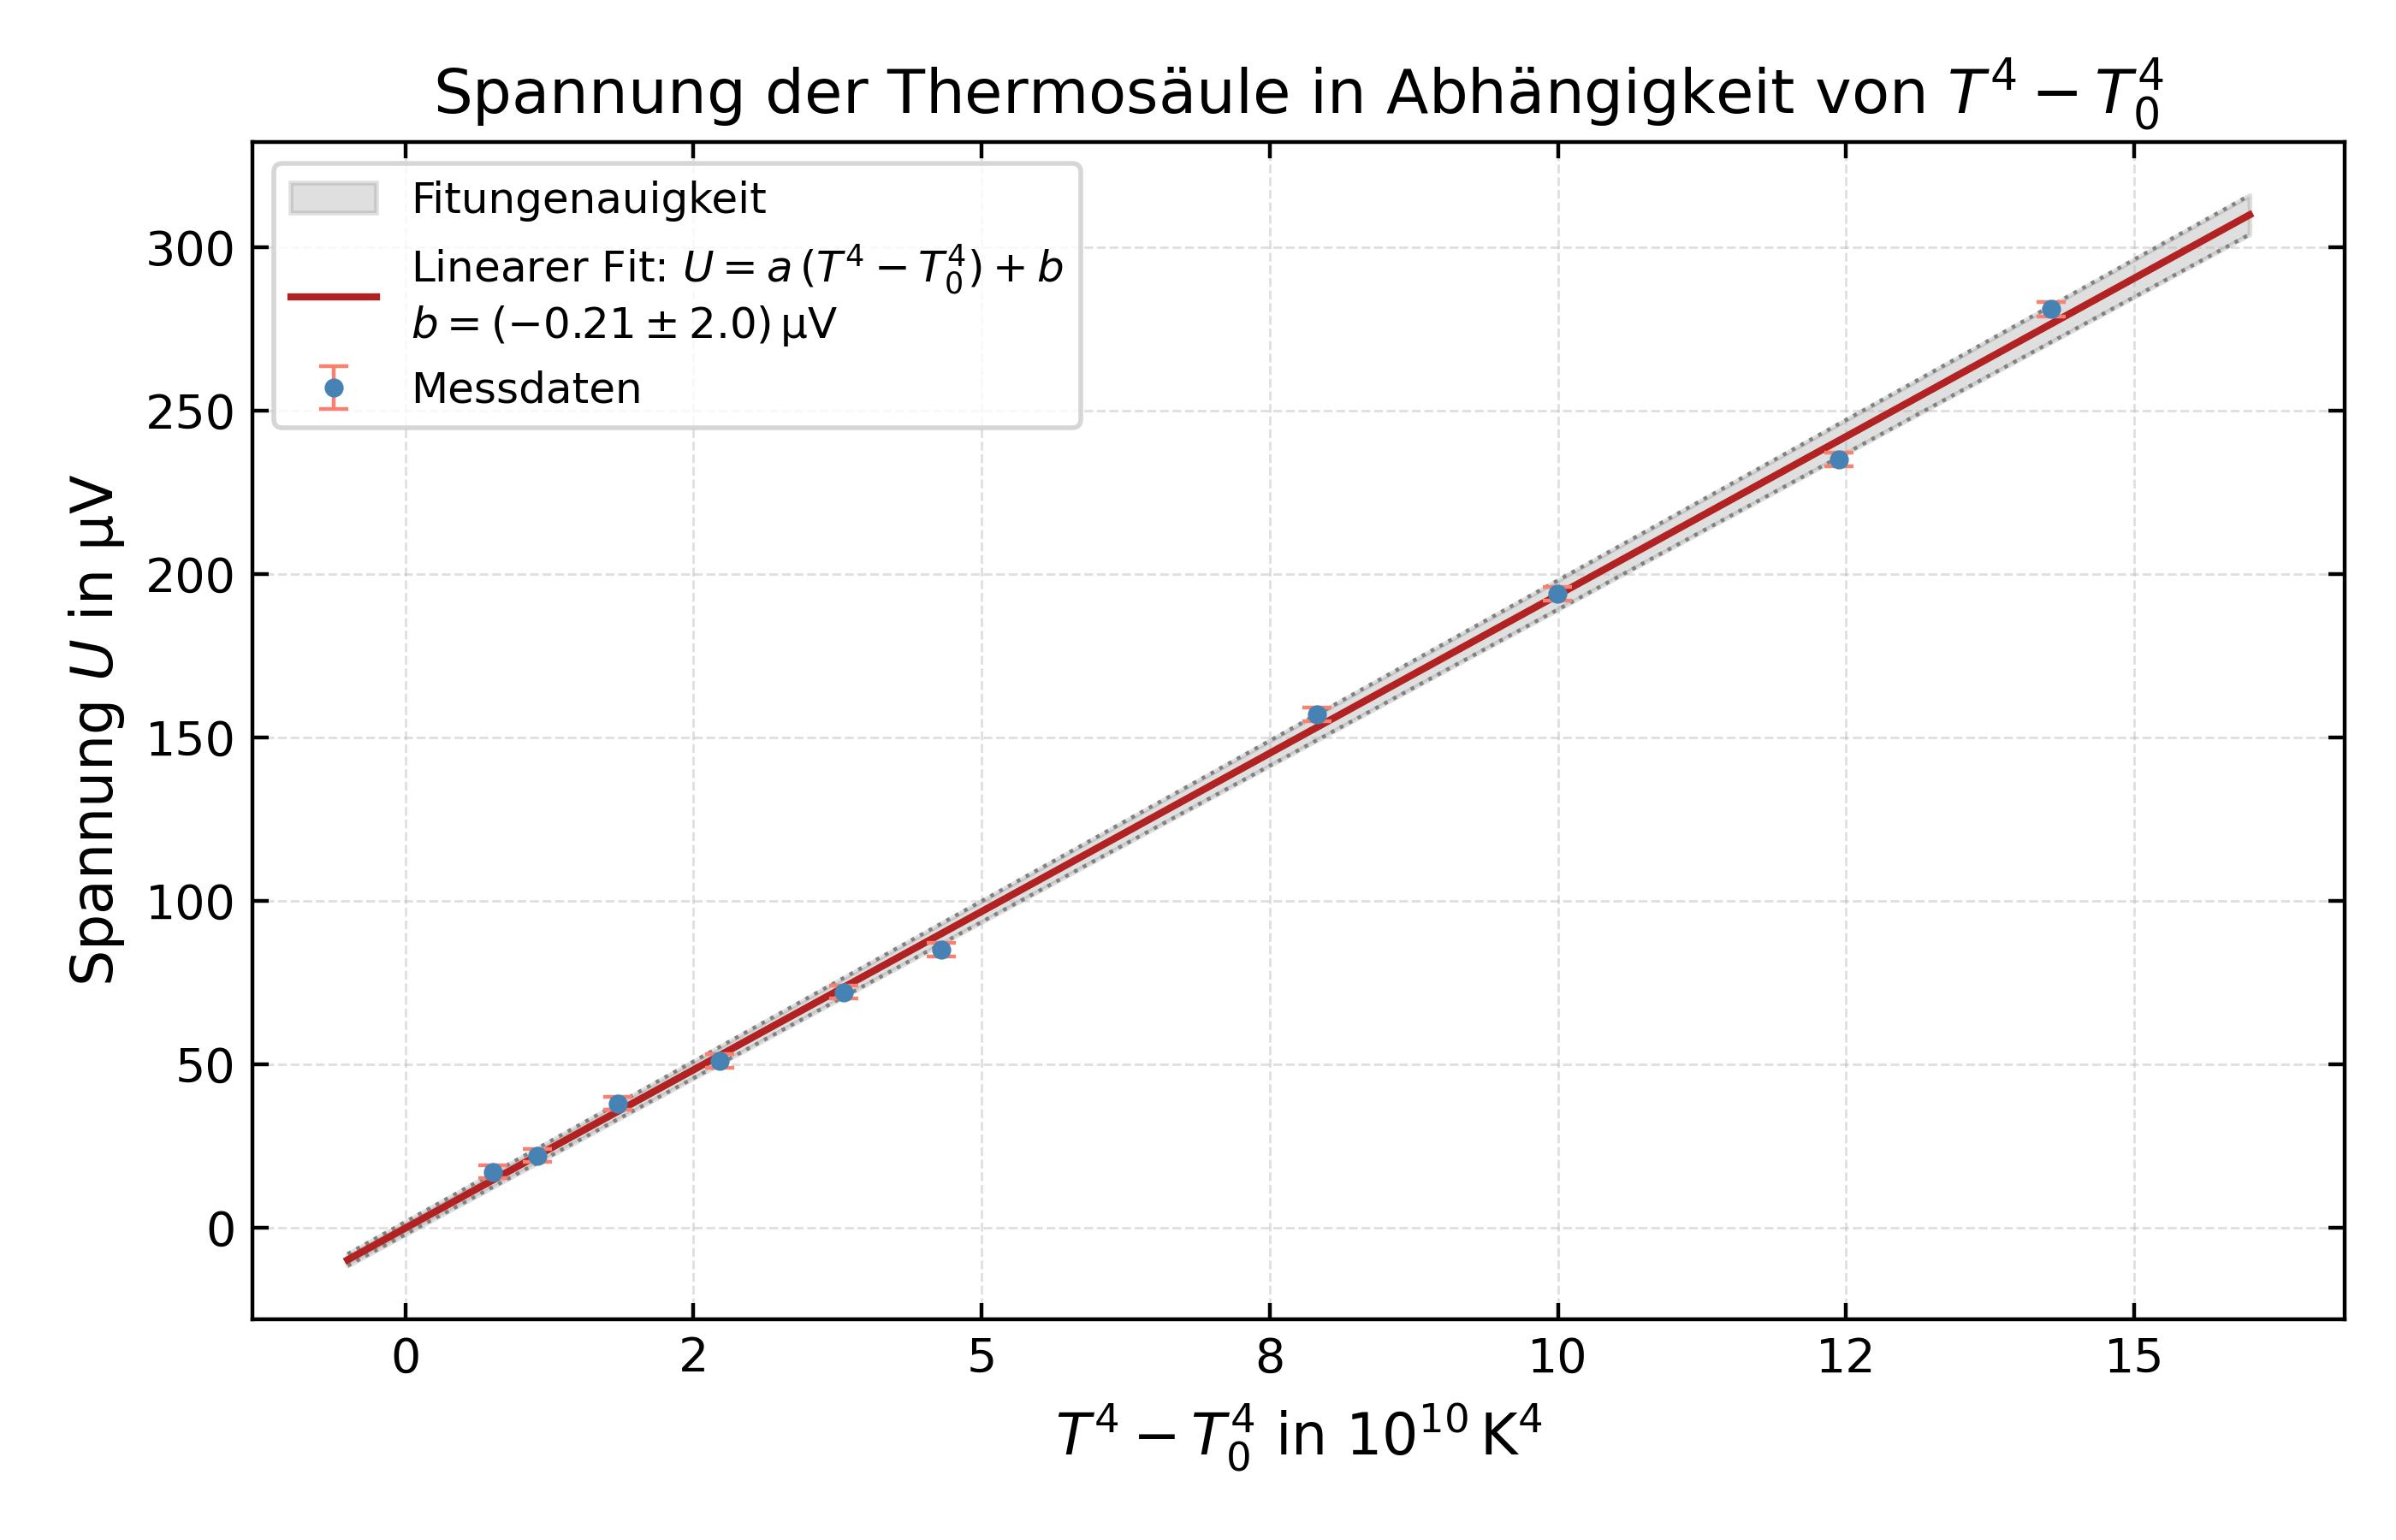
\includegraphics[width=1.4\textwidth]{./Images/TV5_StefanBoltzmann.jpg}
            \caption{$U(T^4-T_0^4)$-Diagramm}
            \label{fig:StefanBoltzmann}
        \end{figure}
    \end{landscape}
\restoregeometry



\newpage
\section{Teilversuch V: Stickstoffeis}
\begin{figure}[H]
            \centering
            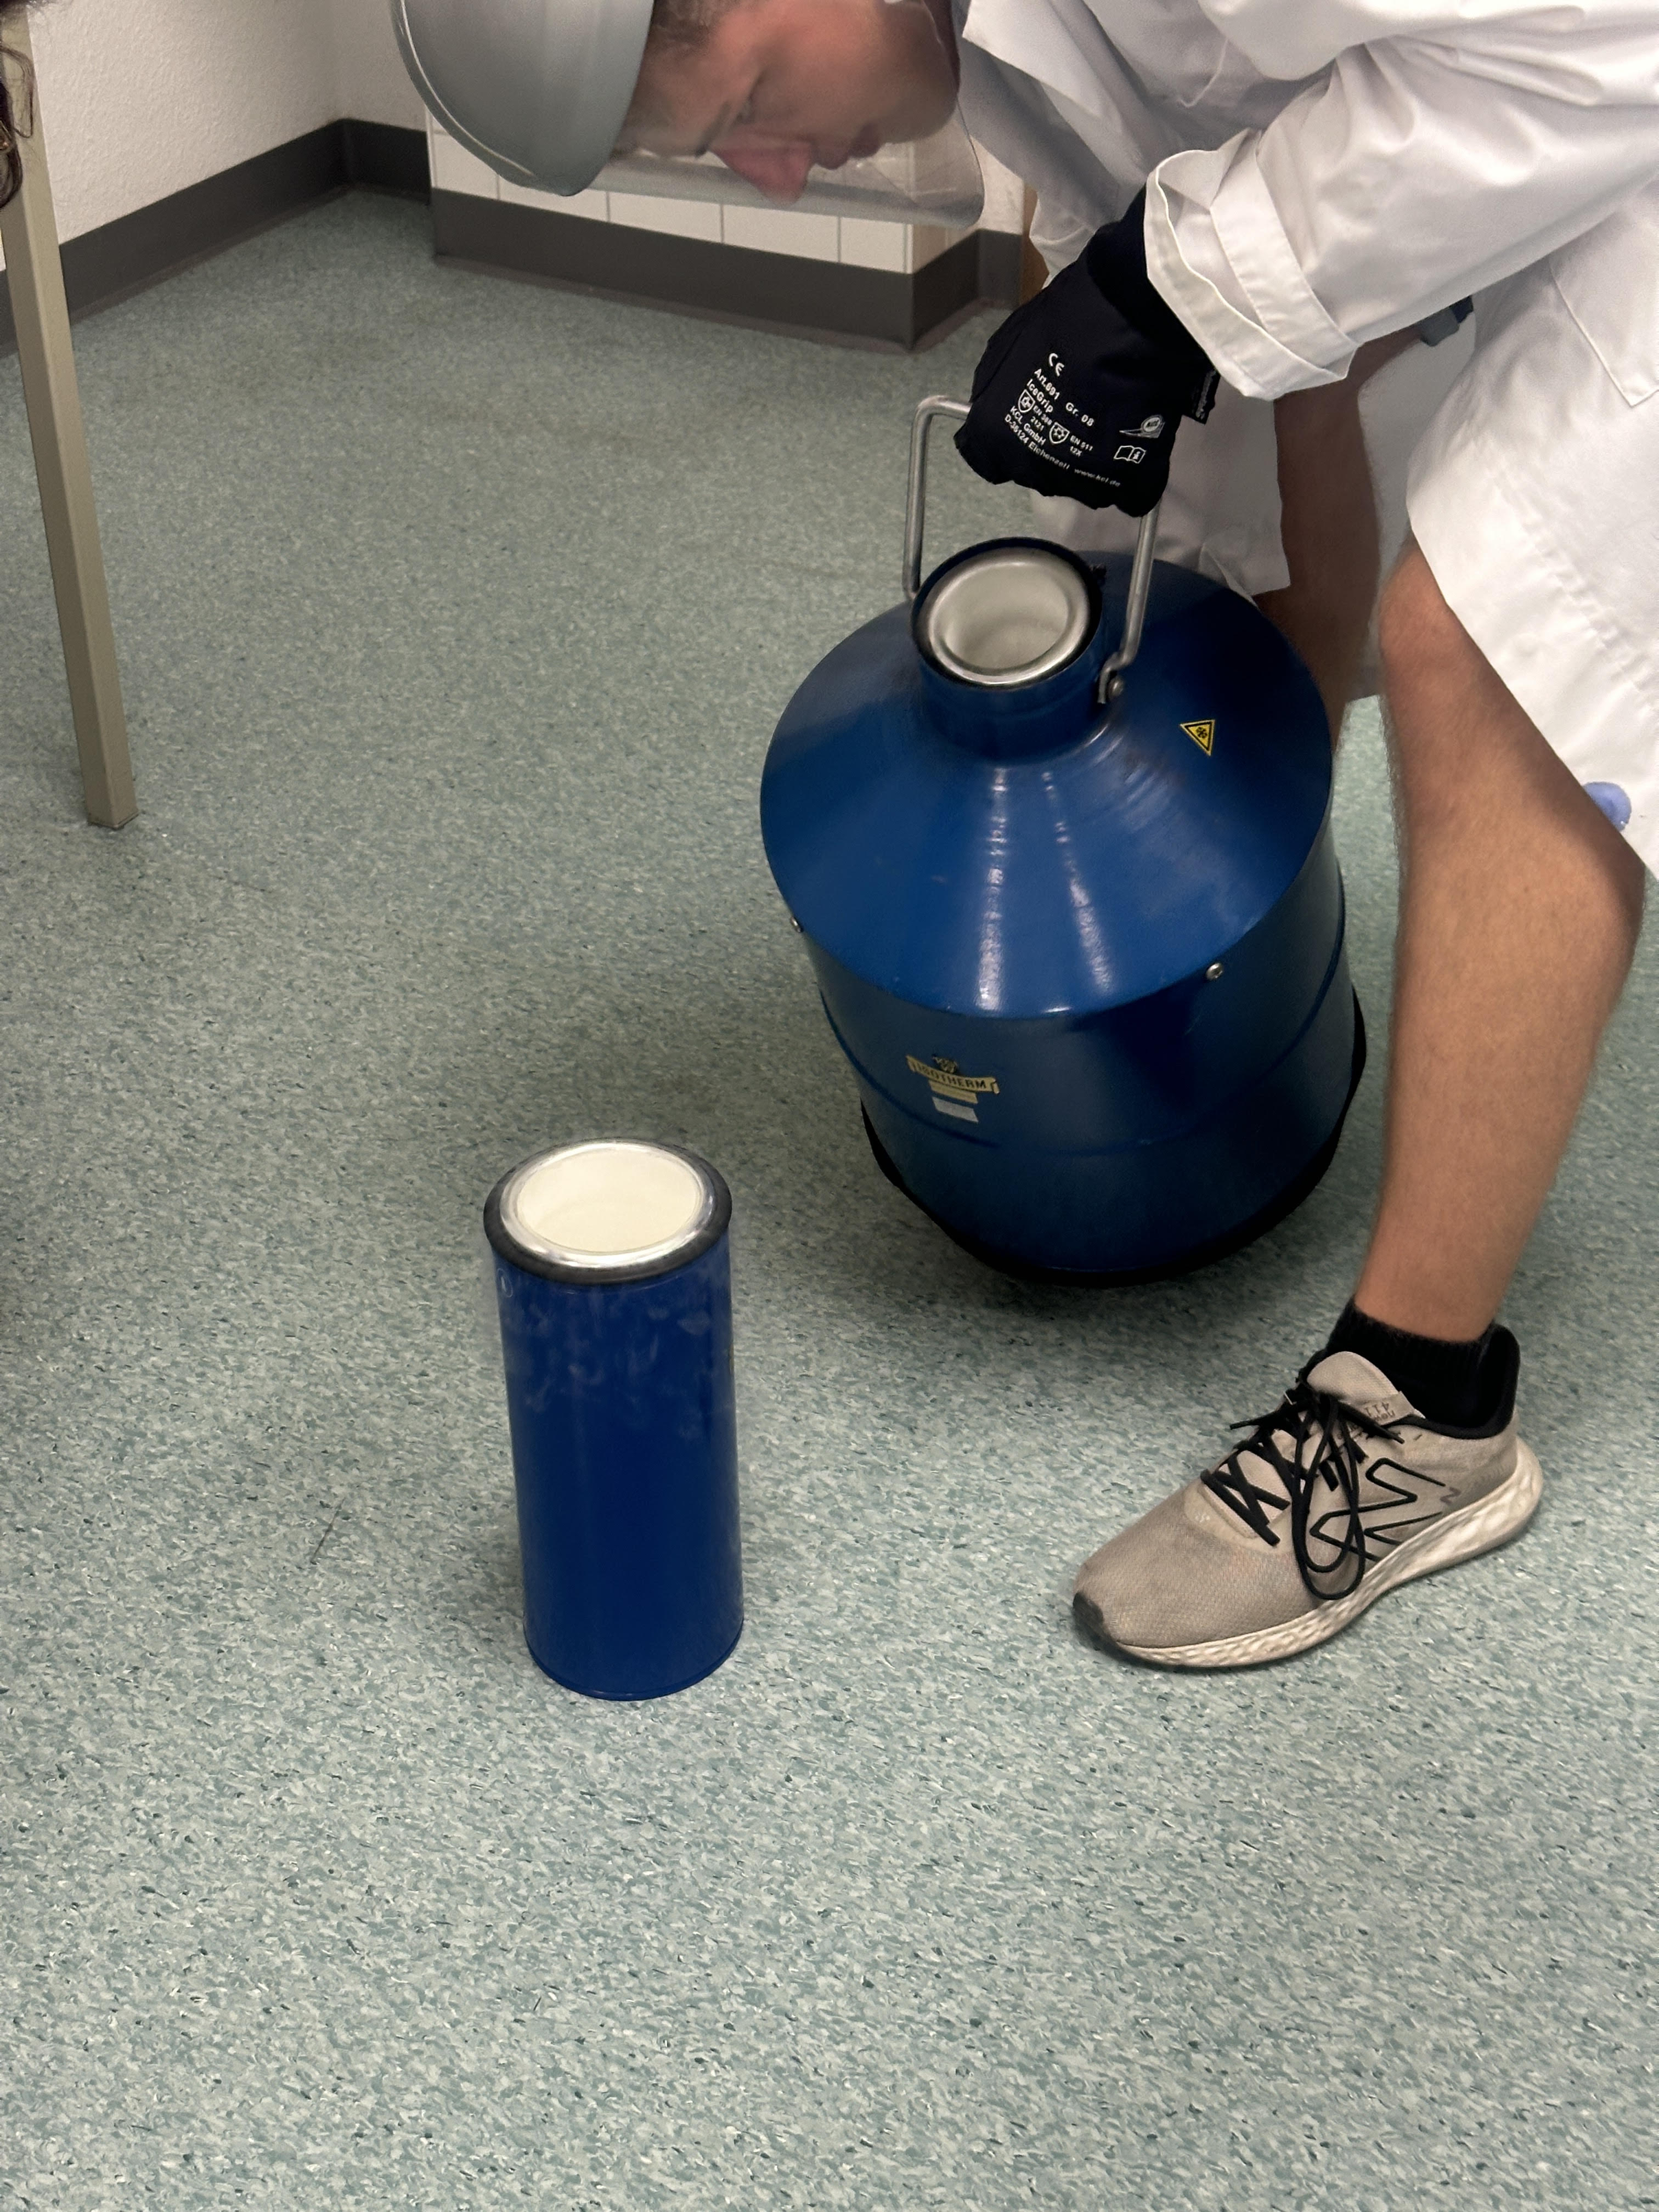
\includegraphics[width=0.8\textwidth]{./Images/unnamed-6.jpg}
            \caption{}
            \label{fig:StefanBoltzmann}
\end{figure}
\begin{figure}[H]
            \centering
            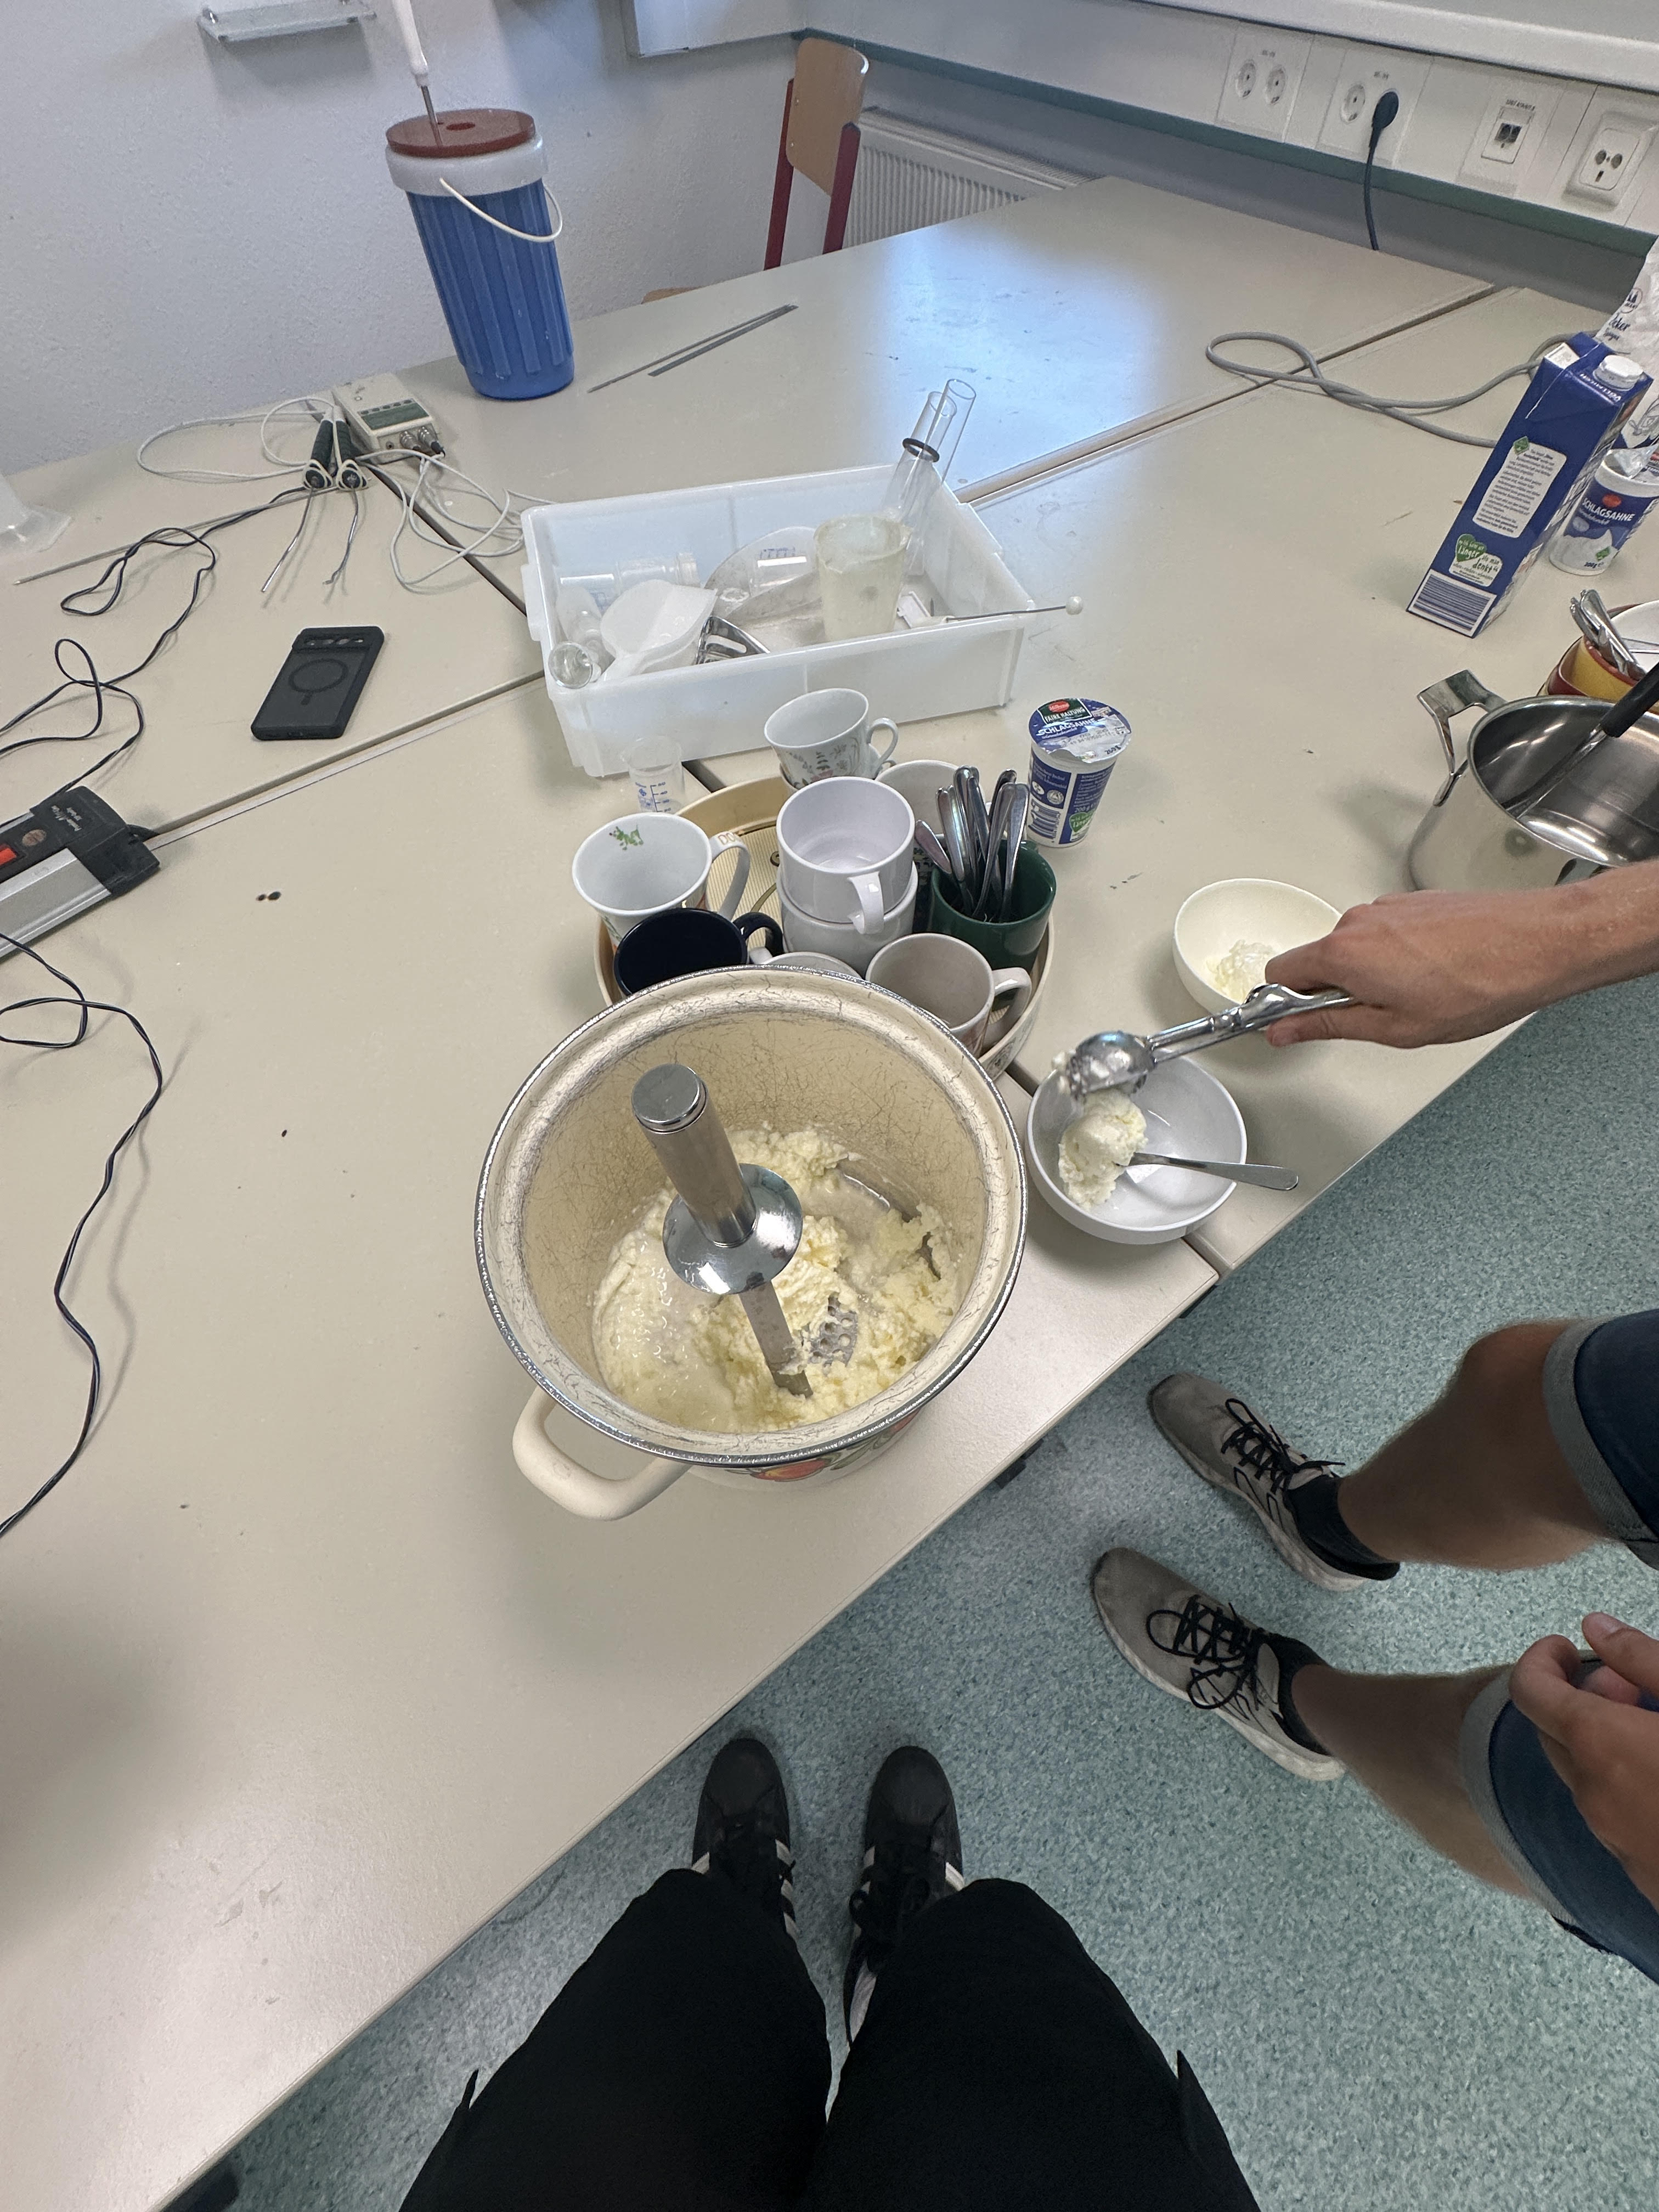
\includegraphics[width=0.8\textwidth]{./Images/unnamed-7.jpg}
            \caption{}
            \label{fig:StefanBoltzmann}
\end{figure}





\newpage
\chapter{Anhang}
\section{Python Scripts}
Die Python Scripts, die zum Plotten der Grafiken verwendet wurden, wurden mit Unterstützung von KI erstellt und dann nach den eigenen Bedürfnissen weiter
bearbeitet.
\definecolor{codegreen}{rgb}{0,0.6,0}
\definecolor{codegray}{rgb}{0.5,0.5,0.5}
\definecolor{codepurple}{rgb}{0.58,0,0.82}
\definecolor{backcolour}{rgb}{0.95,0.95,0.92}

\lstdefinestyle{python}{
    backgroundcolor=\color{backcolour},   
    commentstyle=\color{codegreen},
    keywordstyle=\color{magenta},
    numberstyle=\tiny\color{codegray},
    stringstyle=\color{codepurple},
    basicstyle=\ttfamily\footnotesize,
    breakatwhitespace=false,         
    breaklines=true,                 
    captionpos=b,                    
    keepspaces=true,                 
    numbers=left,                    
    numbersep=5pt,                  
    showspaces=false,                
    showstringspaces=false,
    showtabs=false,                  
    tabsize=2
}
\subsection{TVIII}
\subsubsection{Plotten des Temperaturverlauf während des Gefriervorgangs}
\label{scr:TemperaturverlaufWasserGefrier}
\begin{scriptsize}
\lstset{style=python}
\begin{lstlisting}[language=python]
import numpy as np
import matplotlib.pyplot as plt

temp = [12.68, 10.45, 9.27, 8.05, 7.11, 5.90, 4.88, 3.99, 3.46, 2.82, 2.62, 2.47, 0.61, 0.27, -0.10, -0.18, 0.83, 0.85, 0.03, -0.66, -1.03, -1.60, -1.70, -1.80, -0.11, -0.05]
times = [0, 5, 10, 15, 20, 30, 40, 50, 60, 90, 120, 150, 180, 200, 240, 250, 300, 360, 420, 480, 510, 540, 600, 630, 645, 660]

fig, ax = plt.subplots(figsize=(7, 4.5))
ax.spines['left'].set_position('zero')
ax.spines['bottom'].set_position('zero')
ax.spines['right'].set_visible(False)
ax.spines['top'].set_visible(False)
ax.set_ylabel('Temperatur in C')
ax.set_xlabel('Zeit in s')

plt.plot(times, temp, 'o:r', label = "Gemessene Temperatur")
plt.vlines(150, -3, 13, 'grey', linestyles=':')
plt.text(150, -4, 'Ruehren 1', ha = 'center', size = 7)
plt.vlines(250, -3, 13, 'grey', linestyles=':')
plt.text(250, -4, 'Ruehren 2', ha = 'center', size = 7)
plt.vlines(360, -3, 13, 'grey', linestyles=':')
plt.text(360, -4, 'Ruehren 3', ha = 'center', size = 7)
plt.vlines(630, -3, 13, 'orange')
plt.text(630, -4, 'Kratzen am Glas', ha = 'center', size = 7)
plt.savefig("./04_APW/Images/TV3_TempVerlaufDiag.jpg", dpi = 800)
\end{lstlisting}
\end{scriptsize}

\subsection{TVIV}
\subsubsection{Plot des $p(T)$-Diagramms}
\label{scr:PTDiagramm}
\begin{scriptsize}
\lstset{style=python}
\begin{lstlisting}[language=python]
import numpy as np
import matplotlib.pyplot as plt
from scipy.optimize import curve_fit

temp = np.array([39.9, 50, 80, 90, 100, 105, 110, 115, 120, 125, 130, 135, 140, 145, 150, 155, 160, 165, 170, 175, 180, 185, 190, 195, 200, 205, 210, 215, 220, 225, 230, 235, 240, 245, 250])
temp = temp + 273.15
tempErr = np.full(len(temp), 3)

pressures = np.array([1, 1, 1.9, 2.1, 2.8, 3.0, 3.2, 3.5, 4.0, 4.5, 5.1, 5.4, 6.2, 7.1, 8.0, 9.0, 10.1, 11.1, 12.2, 13.5, 15.0, 16.2, 18.0, 19.8, 21.6, 23.7, 26.0, 28.2, 31.1, 33.3, 36.0, 39.5, 43, 47, 51])
pressures = pressures + 0.965
pressError = np.full(13, 0.5)
pressError = np.append(pressError, np.full(len(pressures) - 13, 1))

def func(T, a, b, c):
    return a + np.exp(c + b / T)

params, covariance = curve_fit(func, temp, pressures)
a, b, c = params
perr = np.sqrt(np.diag(covariance))  # Unsicherheiten der Parameter

temp_fit = np.linspace(min(temp), max(temp), 500)
press_fit = func(temp_fit, a, b, c)

fig, ax = plt.subplots(figsize=(7, 4.5))

ax.errorbar(temp, pressures, pressError, tempErr,
            fmt='o', color='steelblue', ecolor='salmon',
            ms=3, capsize=3, label='Messdaten')

ax.plot(temp_fit, press_fit, 'r-', linewidth=1.5,
        label=(f'Fit: $a + e^{{c + b/T}}$\n'
               f'$a = ({a:.3f} \\pm {perr[0]:.3f})$bar'))

ax.set_ylabel('Druck in bar')
ax.set_xlabel('Temperatur in K')
ax.set_title('Dampfdruckkurve')
ax.legend(fontsize=9)
ax.grid(True, linestyle='--', alpha=0.4)

plt.tight_layout()
# plt.show()
plt.savefig("./04_APW/Images/PTDiagramm.jpg", dpi = 400)
\end{lstlisting}
\end{scriptsize}
\newpage
\subsubsection{Plot des $-1/T^2$-$\ln(p)$-Diagramms}
\label{scr:lnPTDiagramm}
\begin{scriptsize}
\lstset{style=python}
\begin{lstlisting}[language=python]
import numpy as np
import matplotlib.pyplot as plt
from math import ceil

# --- Temperatur ---
temp_C = np.array([80, 90, 100, 105, 110, 115, 120, 125, 130, 135,
                   140, 145, 150, 155, 160, 165, 170, 175, 180, 185, 190, 195,
                   200, 205, 210, 215, 220, 225, 230, 235, 240, 245, 250])
temp = temp_C + 273.15
tempErr = np.full(len(temp), 3)
xVals  = -1 / temp
xError = tempErr / temp**2
# --- Druck ---
pressures_raw = np.array([1.9, 2.1, 2.8, 3.0, 3.2, 3.5, 4.0, 4.5, 5.1, 5.4,
                           6.2, 7.1, 8.0, 9.0, 10.1, 11.1, 12.2, 13.5, 15.0, 16.2,
                           18.0, 19.8, 21.6, 23.7, 26.0, 28.2, 31.1, 33.3, 36.0,
                           39.5, 43, 47, 51])
pressures = pressures_raw + 0.965 - 1.798

pressError = np.concatenate([np.full(13, 0.5), np.full(len(pressures) - 13, 1.0)])
lnPressures = np.log(pressures)
lnPressError = pressError / pressures

# --- Fit ---
line, cov = np.polyfit(xVals, lnPressures, 1, cov=True)
slope, intercept = line
dSlope, dIntercept = np.sqrt(np.diag(cov))
yline = np.polyval(line, xVals)
labelFit = (rf"Linearer Fit: $ln(p/bar) = a \cdot (-1/T) + b$" "\n" rf"$a = ({round(slope)} \pm {ceil(dSlope)})K$")

# --- Plot ---
fig, ax = plt.subplots(figsize=(7, 4.5))

ax.errorbar(
    xVals, lnPressures,
    yerr=lnPressError, xerr=xError,
    fmt='o', color='steelblue', ecolor='salmon',
    ms=3, capsize=3, label='Messdaten'
)

ax.plot(
    xVals, yline,
    color = 'grey',
    linewidth=1.5,
    label=labelFit,
)

ax.set_xlabel(r"$-1/T$ in $\mathrm{K^{-1}}$")
ax.set_ylabel(r"$\ln(p\,/\,\mathrm{bar})$")
ax.set_title(r"$-1/T$ - $ln(p)$-Diagramm")
ax.legend(fontsize=9)
ax.grid(True, linestyle='--', alpha=0.4)

plt.tight_layout()
plt.savefig("./04_APW/Images/TV4_lnPTDiagrammValsRemoved.jpg", dpi=400)
plt.show()
\end{lstlisting}
\end{scriptsize}
\newpage
\subsection{TVV}
\subsubsection{Plot des $U(T^4-T_0^4)$-Diagramms}
\label{scr:StefanBoltzmannDiagramm}
\begin{scriptsize}
\lstset{style=python}
\begin{lstlisting}[language=python]
import numpy as np
from matplotlib import pyplot as plt
from math import ceil
# --- Daten ---
T = np.array([80, 100, 130, 160, 190, 210, 270, 300, 330, 350]) + 273.15
T0 = 25.6 + 273.15
xVals = T**4 - T0**4

U = np.array([17, 22, 38, 51, 72, 85, 157, 194, 235, 281])
dU = 0.0004 * U + 2

# --- Fit ---
line, cov = np.polyfit(xVals, U, 1, cov=True)
slope, intercept = line
dSlope, dIntercept = np.sqrt(np.diag(cov))

xFit = np.linspace(-0.05e11, 1.6e11, 300)
yFit    = slope * xFit + intercept
yFitUp  = (slope + dSlope) * xFit + (intercept + dIntercept)
yFitLow = (slope - dSlope) * xFit + (intercept - dIntercept)

print(f"Achsenabschnitt b = ({intercept:.3f} \pm {dIntercept:.3f}) muV")
print(f"Steigung      a = ({slope:.3e} \pm {dSlope:.3e}) muV/K^4")

# --- Plot ---
fig, ax = plt.subplots(figsize=(7, 4.5))

# Fehlerband
ax.fill_between(xFit, yFitLow, yFitUp,
                color='grey', alpha=0.25, label='Fitungenauigkeit')

# Grenzlinien
ax.plot(xFit, yFitUp,  color='grey', linewidth=0.8, linestyle=':')
ax.plot(xFit, yFitLow, color='grey', linewidth=0.8, linestyle=':')

# Fit
ax.plot(xFit, yFit, color='firebrick', linewidth=1.5,
        label=(rf'Linearer Fit: $U = a\,(T^4 - T_0^4) + b$'
               '\n'
               rf'$b = ({round(intercept, 2)} \pm {ceil(dIntercept*10)/10})\,\mathrm{{\mu V}}$'))

# Messdaten
ax.errorbar(
    xVals, U, yerr=dU,
    fmt='o', color='steelblue', ecolor='salmon',
    ms=3, capsize=3, linewidth=0,
    elinewidth=0.8, capthick=0.8,
    label='Messdaten', zorder=5
)

ax.set_xlabel(r'$T^4 - T_0^4$ in $\mathrm{K^4}$', fontsize=12)
ax.set_ylabel(r'Spannung $U$ in $\mathrm{\mu V}$', fontsize=12)
ax.set_title(r'Spannung der Thermosaeule in Abhaengigkeit von $T^4 - T_0^4$', fontsize=13)

ax.tick_params(direction='in', top=True, right=True)
ax.grid(True, linestyle='--', linewidth=0.5, alpha=0.4)
ax.legend(fontsize=9)

# x-Achse in 10^10 skalieren
ax.xaxis.set_major_formatter(
    plt.FuncFormatter(lambda x, _: f'{x/1e10:.0f}')
)
ax.set_xlabel(r'$T^4 - T_0^4$ in $10^{10}\,\mathrm{K^4}$', fontsize=12)

fig.tight_layout()
plt.savefig("./04_APW/Images/TV5_StefanBoltzmann.jpg", dpi=400)
plt.show()
\end{lstlisting}
\end{scriptsize}

\end{document}
